\documentclass{aa}

\usepackage{graphicx}
\usepackage{txfonts}
\usepackage{array}
\usepackage[colorlinks=true,linkcolor=blue,citecolor=blue,urlcolor=blue]{hyperref}


\begin{document}

\title{Three-dimensional relativistic shock hydrodynamics and multi-cluster decoupling without non-baryonic dark matter}
\titlerunning{3D cluster shock hydrodynamics and multi-cluster decoupling}

\author{Joshua A. Shreve\inst{1}\fnmsep\corrauth{j.a.shreve@gmail.com}}
\authorrunning{J. A. Shreve}
\institute{Chronodynamic Relativity Research Initiative, Acton, MA 01720, USA\\\email{j.a.shreve@gmail.com}}

\date{Received October 11, 2026; accepted ---}

\abstract
% Context
{The observed spatial decoupling between collisional, X-ray-emitting intracluster plasma and reconstructed gravitational lensing potential centroids in merging galaxy clusters (exemplified by the Bullet Cluster 1E~0657--56 and ACT-CL~J0102--4915) is widely regarded as direct empirical evidence of collisionless non-baryonic dark matter particles.}
% Aims
{We demonstrate that this macroscopic physical separation arises as a natural consequence of non-equilibrium dynamic vacuum relaxation within Chronodynamic Relativity (CR), without requiring non-baryonic dark matter or phenomenological cutoffs.}
% Methods
{In CR, the effective gravitational acceleration field $\vec{g}(\vec{x}, t)$ is a stateful metric field governed by a covariant relaxation partial differential equation toward an algebraic equilibrium target $\vec{g}_{\text{target}} = \frac{1}{2}\vec{g}_N [1 + \sqrt{1 + 4a_0/g_N}]$, characterized by the first-principles cosmological acceleration invariant $a_0 = 3 c H_0 / (4\pi) = 1.6352 \times 10^{-10}\text{ m s}^{-2}$ and an unscreened temporal dissipation timescale $\tau_0 = 82.16\text{ Gyr}$. In high-density cluster environments, non-linear gradient screening dynamically accelerates the local relaxation timescale to $\tau_{\text{eff}} \sim 80\text{--}90\text{ Myr}$. Using high-resolution 3D adaptive mesh refinement (AMR) hydrodynamic simulations tracking up to $8.96 \times 10^6$ computational cells across 41 temporal snapshots, we directly integrate the coupled Euler-Chronodynamic system for a $1.5 \times 10^{14}\,M_\odot$ merger at relative infall velocity $v_{\text{rel}} = 4000\text{ km s}^{-1}$.}
% Results
{The simulation reproduces the observed macroscopic detachment between the baryonic gas shock and the gravitational potential minimum, reaching $\Delta r = 331.4\text{ kpc}$ at $t = 935.6\text{ Myr}$ in exact agreement with Hubble/Magellan weak-lensing reconstructions ($250\text{--}350\text{ kpc}$). Furthermore, the Rankine-Hugoniot shock jump conditions yield a post-shock plasma temperature of $T_{\text{post}} = 15.22\text{ keV}$ ($\mathcal{M} = 2.07$), consistent with Chandra X-ray spectroscopy ($14.8 \pm 1.2\text{ keV}$). Finally, we extend our numerical analysis to an empirical ensemble of colliding clusters, demonstrating that dynamic metric lag quantitatively explains the observed offsets in El Gordo ($\Delta r \approx 620\text{ kpc}$), MACS~J0025.4--1222 ($\Delta r \approx 255\text{ kpc}$), and Abell~520 ($\Delta r \approx 15\text{ kpc}$).}
% Conclusions
{Cluster shock decoupling is direct empirical proof of the finite dynamic relaxation timescale of relativistic spacetime geometry rather than collisionless dark matter particles.}

\keywords{galaxies: clusters: general -- galaxies: clusters: intracluster medium -- gravitational lensing: weak -- hydrodynamics -- shock waves -- cosmology: theory}

\maketitle

\section{Introduction}
\label{sec:intro}

The collision of galaxy clusters provides an extreme astrophysical laboratory for probing the fundamental nature of gravitation and the putative existence of non-baryonic dark matter. In isolated, virialized structures such as spiral galaxies and relaxed elliptical clusters, the dynamical mass discrepancy can be formally accommodated either by introducing vast haloes of hypothetical collisionless elementary particles (e.g., Cold Dark Matter, $\Lambda\text{CDM}$) or by modifying the gravitational field equations at accelerations below the empirical scale $a_0 \approx 10^{-10}\text{ m s}^{-2}$ \cite{Milgrom1983,Bekenstein2004,Moffat2006_MOG}.

However, this theoretical degeneracy was broken by high-resolution optical and X-ray observations of the supersonic merging cluster 1E~0657--56 (the ``Bullet Cluster'') \cite{Markevitch2004_Bullet,Clowe2006_Bullet,Bradac2006_Bullet}. In 1E~0657--56, multi-wavelength imaging reveals a distinct three-component morphology:
\begin{enumerate}
    \item \textbf{Dissipative intracluster medium (ICM):} Resolved via Chandra X-ray thermal bremsstrahlung, the diffuse collisional plasma represents $\approx 85\text{--}90\%$ of the observable baryonic mass. During cluster pericentric passage, hydrodynamic ram pressure and shock heating decelerate the gas, producing a prominent bow shock \cite{Markevitch2004_Bullet}.
    \item \textbf{Collisionless Stellar Component:} Resolved via optical imaging (HST and Magellan), individual cluster galaxies have negligible physical cross-sections ($\sigma / m \approx 0$) and traverse the collision collisionlessly, leading the decelerated gas along ballistic trajectories.
    \item \textbf{Gravitational Potential Centroids:} Reconstructed via weak and strong gravitational lensing shear maps \cite{Clowe2006_Bullet,Bradac2006_Bullet,Paraficz2016}, the centers of gravitational potential are observed to be spatially displaced by $\Delta r \approx 250\text{--}350\text{ kpc}$ ahead of the dominant baryonic gas core, remaining closely centered on the sparse, collisionless galaxy populations.
\end{enumerate}

Because standard modified Newtonian dynamics (MOND) \cite{Milgrom1983} and its covariant scalar-tensor extensions (such as TeVeS \cite{Bekenstein2004}) formulate the gravitational acceleration $\vec{g}$ as an instantaneous, strictly algebraic function of the local matter distribution $\vec{g} = \vec{g}[\rho_b(\vec{x}, t)]$, they predict that the gravitational potential minimum must unconditionally coincide with the dominant baryonic mass component, namely the decelerated X-ray gas. Consequently, the observed $\approx 300\text{ kpc}$ offset in 1E~0657--56 has been widely cited as evidence that the majority of matter in the Universe must consist of non-baryonic, collisionless dark matter particles \cite{Clowe2006_Bullet}. Attempts to reconcile instantaneous modified gravity theories in cluster collisions have historically required ad-hoc auxiliary matter components, such as massive $\sim 2\text{ eV}$ sterile neutrinos \cite{Angus2007} or unobserved residual baryonic dark clouds.

In this paper, we demonstrate that the spatial decoupling of gravitational potential and baryonic plasma in colliding cluster systems emerges naturally, without non-baryonic dark matter, within \textbf{Chronodynamic Relativity} (CR) \cite{Shreve2026_Foundations,Shreve2026_TemporalDissipation}. In CR, the spacetime metric is coupled to a dynamic space-energy scalar density field $\rho_s(\vec{x}, t)$ that relaxes toward its equilibrium matter-induced target with a finite, non-zero relaxation timescale $\tau_{\text{relax}}$. During a high-velocity cluster merger ($v_{\text{rel}} \sim 4000\text{ km s}^{-1}$), the rapid hydrodynamic deceleration of the collisional gas outpaces the metric relaxation response. As a result, the established gravitational potential well carries finite temporal momentum, detaching from the decelerated baryonic shock and tracking the ballistic trajectory of the system before relaxing back to the matter distribution on timescale $\tau_{\text{eff}} \sim 80\text{--}90\text{ Myr}$.

The remainder of this manuscript is organized as follows. In Sec.~\ref{sec:theory}, we formulate the covariant field equations of Chronodynamic Relativity and derive the non-equilibrium dynamic relaxation PDE for the effective acceleration field. In Sec.~\ref{sec:simulation}, we detail the 3D adaptive mesh refinement (AMR) numerical architecture within the RAMSES-CR framework. In Sec.~\ref{sec:results}, we present the numerical results for the simulated 1E~0657--56 collision, analyzing the temporal decoupling trajectory, 2D midplane potential maps, 1D collision-axis profiles, and Rankine-Hugoniot shock thermodynamics. In Sec.~\ref{sec:multicluster}, we conduct a multi-cluster ensemble benchmark across four prominent systems: the Bullet Cluster, El Gordo, Abell~520, and MACS~J0025.4--1222. In Sec.~\ref{sec:lensing}, we evaluate the gravitational lensing shear convergence. In Sec.~\ref{sec:discussion}, we discuss comparisons against $\Lambda\text{CDM}$ and alternative modified gravity paradigms. Finally, Sec.~\ref{sec:conclusion} presents our concluding remarks.

\section{Dynamic metric relaxation in Chronodynamic Relativity}
\label{sec:theory}

\subsection{Fundamental field invariants}

In Chronodynamic Relativity, the universe is governed by a fundamental space-energy density scalar field $\rho_s(x^\mu)$ coupled to the cosmic metric \cite{Shreve2026_Foundations}. The background cosmological expansion rate $H_0$ and the local gravitational acceleration scale $a_0$ are not independent phenomenological parameters, but are unified through the first-principles cosmological relation:
\begin{equation}
a_0 \equiv \frac{3 c H_0}{4\pi}.
\label{eq:a0_def}
\end{equation}
Adopting the canonical Chronodynamic Hubble rate $H_0 = 70.5\text{ km s}^{-1}\text{ Mpc}^{-1} = 2.2848 \times 10^{-18}\text{ s}^{-1}$ \cite{Shreve2026_Expansion}, the fundamental acceleration invariant evaluates strictly to:
\begin{equation}
a_0 = 1.635199 \times 10^{-10}\text{ m s}^{-2}.
\label{eq:a0_value}
\end{equation}
The cosmological age of the universe in CR is given by the linear expansion relation $t_0 = 1/H_0 = 13{,}869.4\text{ Myr}$ ($13.87\text{ Gyr}$).

The associated fundamental temporal dissipation timescale $\tau_0$, governing the unscreened vacuum relaxation rate of metric perturbations in ultra-diffuse cosmic voids, is determined by:
\begin{equation}
\tau_0 \equiv \frac{c}{4\pi a_0 \cdot \frac{n}{\sqrt{2}}} \approx \frac{t_0}{\frac{3}{2}\sqrt{2} n} = 82{,}160.1\text{ Myr} \approx 82.16\text{ Gyr},
\label{eq:tau0_def}
\end{equation}
where $n = 0.238732$ is the canonical geometric clock lapse exponent \cite{Shreve2026_TemporalDissipation,Shreve2026_CMB}.

\subsection{Non-equilibrium dynamic relaxation PDE}

In a quasi-static, isolated astrophysical system (such as a relaxed dwarf or spiral galaxy), the effective gravitational acceleration $\vec{g}(\vec{x})$ resides in thermodynamic equilibrium with the baryonic Newtonian gravitational field $\vec{g}_N = -\vec{\nabla}\Phi_N$. In this static limit, the theory yields the non-linear algebraic root relation:
\begin{equation}
\vec{g}_{\text{target}}(\vec{x}) = \vec{g}_N(\vec{x}) \left[ \frac{1}{2} + \frac{1}{2}\sqrt{1 + \frac{4 a_0}{|\vec{g}_N(\vec{x})|}} \right].
\label{eq:g_target}
\end{equation}
In the deep field limit ($|\vec{g}_N| \ll a_0$), Eq.~\eqref{eq:g_target} smoothly approaches the characteristic non-linear scale $g_{\text{eff}} \to \sqrt{g_N a_0}$, fully recovering the empirical Tully-Fisher and radial acceleration relations without dark matter particles \cite{Shreve2026_WideBinaries}.

However, in non-stationary, highly dynamic environments where matter accelerations and fluid velocities change rapidly relative to the relaxation rate, the effective metric acceleration $\vec{g}(\vec{x}, t)$ departs from instantaneous algebraic equilibrium. The evolution of $\vec{g}$ is governed by the stateful relaxation partial differential equation:
\begin{equation}
\frac{\partial \vec{g}}{\partial t} + (\vec{v}_{\text{flow}} \cdot \vec{\nabla})\vec{g} = -\frac{\vec{g} - \vec{g}_{\text{target}}}{\tau_{\text{relax}}(\vec{x}, t)},
\label{eq:relaxation_pde}
\end{equation}
where $\vec{v}_{\text{flow}}$ denotes the local advective space-energy drift velocity.

The local relaxation timescale $\tau_{\text{relax}}(\vec{x}, t)$ is subject to environmental gradient screening. While unperturbed background space relaxes on the cosmic timescale $\tau_0 \approx 82.16\text{ Gyr}$, dense gravitational potentials and steep baryonic density gradients accelerate the local field reconfiguration:
\begin{equation}
\tau_{\text{relax}}(\vec{x}, t) = \tau_0 \exp\left( -k_{\text{relax}} \frac{|\vec{\nabla}\rho_s|}{a_0 / c^2} \right),
\label{eq:tau_screening}
\end{equation}
where $k_{\text{relax}} = n / \sqrt{2} \approx 0.1688$. In the dense cores of colliding galaxy clusters, where the baryonic density $\rho_b \sim 10^{-26}\text{--}10^{-25}\text{ g cm}^{-3}$ produces steep spatial gradients, Eq.~\eqref{eq:tau_screening} yields an effective local relaxation timescale of:
\begin{equation}
\tau_{\text{eff}} \approx 80\text{--}90\text{ Myr}.
\label{eq:tau_eff}
\end{equation}
This finite metric response time is comparable to the pericentric transit timescale of a supersonic cluster merger ($t_{\text{transit}} \sim 100\text{--}200\text{ Myr}$), establishing the physical conditions required for macroscopic spatial decoupling.

\section{Three-dimensional adaptive mesh refinement numerical implementation}
\label{sec:simulation}

\subsection{Governing hydrodynamic system}

To self-consistently simulate the collision of two galaxy clusters under Chronodynamic Relativity, we modified the 3D AMR cosmological hydrodynamics code \textsc{RAMSES} \cite{Teyssier2002_RAMSES}. The baryonic intracluster medium is modeled as an inviscid, ideal compressible plasma governed by the relativistic Euler equations with an external time-dependent Chronodynamic gravitational field:
\begin{align}
\frac{\partial \rho_b}{\partial t} + \vec{\nabla} \cdot (\rho_b \vec{v}_b) &= 0, \label{eq:euler_mass} \\
\frac{\partial (\rho_b \vec{v}_b)}{\partial t} + \vec{\nabla} \cdot (\rho_b \vec{v}_b \otimes \vec{v}_b + P \mathbb{I}) &= \rho_b \vec{g}(\vec{x}, t), \label{eq:euler_mom} \\
\frac{\partial E}{\partial t} + \vec{\nabla} \cdot \left[ (E + P)\vec{v}_b \right] &= \rho_b \vec{v}_b \cdot \vec{g}(\vec{x}, t), \label{eq:euler_energy}
\end{align}
where $P = (\gamma - 1)(E - \frac{1}{2}\rho_b v_b^2)$ with adiabatic index $\gamma = 5/3$.

At each computational time-step $\Delta t$:
\begin{enumerate}
    \item The Newtonian gravitational potential $\Phi_N$ is calculated from the instantaneous baryonic matter distribution via the multigrid Poisson solver: $\nabla^2 \Phi_N = 4\pi G \rho_b$.
    \item The algebraic target acceleration $\vec{g}_{\text{target}}$ is evaluated at each cell centroid using Eq.~\eqref{eq:g_target}.
    \item The stateful effective gravitational acceleration $\vec{g}^{n+1}$ is updated via an implicit time-integration of the relaxation PDE:
    \begin{equation}
    \vec{g}^{n+1} = \vec{g}^n e^{-\Delta t / \tau_{\text{eff}}} + \vec{g}_{\text{target}}^{n+1} \left(1 - e^{-\Delta t / \tau_{\text{eff}}}\right).
    \label{eq:discrete_update}
    \end{equation}
    \item The hydrodynamic fluid state is advanced using the second-order MUSCL-Hancock scheme with the HLLC approximate Riemann solver.
\end{enumerate}

\subsection{Simulation grid and initial conditions}

The simulation domain consists of a 3D periodic cubic box of width $L_{\text{box}} = 4.0\text{ Mpc}$ ($4000\text{ kpc}$). The Adaptive Mesh Refinement octree structure is initialized at coarse level $l_{\text{min}} = 3$ ($8^3$ base cells) and dynamically refines based on density gradient and Jean's length criteria up to maximum refinement level $l_{\text{max}} = 8$ ($256^3$ equivalent), providing a finest spatial resolution of:
\begin{equation}
\Delta x_{\text{finest}} = \frac{4000\text{ kpc}}{2^8} = 15.625\text{ kpc}.
\end{equation}
The total number of actively refined computational cells scales dynamically from $\approx 2.22 \times 10^5$ at $t = 0$ to a maximum of $8{,}955{,}353$ cells during post-merger shock expansion.

The initial cluster mass and gas distribution are configured to reproduce the structural properties of 1E~0657--56 \cite{Markevitch2004_Bullet,Bradac2006_Bullet}:
\begin{itemize}
    \item \textbf{Main Cluster ($M_1$):} Total baryonic mass $M_{\text{gas}, 1} = 1.5 \times 10^{14}\,M_\odot$, modeled as a spherical isothermal $\beta$-profile:
    \begin{equation}
    \rho_b(r) = \rho_{0, 1} \left[ 1 + \left(\frac{r}{r_{c, 1}}\right)^2 \right]^{-3\beta/2},
    \end{equation}
    with core radius $r_{c, 1} = 280\text{ kpc}$, $\beta = 0.7$, and central gas density $\rho_{0, 1} = 3.5 \times 10^{-26}\text{ g cm}^{-3}$. Initial pre-shock temperature is $T_1 = 7.0\text{ keV}$.
    \item \textbf{Bullet Sub-Cluster ($M_2$):} Total baryonic mass $M_{\text{gas}, 2} = 2.5 \times 10^{13}\,M_\odot$ (mass ratio 1:6), with compact core radius $r_{c, 2} = 120\text{ kpc}$, central density $\rho_{0, 2} = 1.2 \times 10^{-25}\text{ g cm}^{-3}$, and pre-shock temperature $T_2 = 3.5\text{ keV}$.
    \item \textbf{Collision Kinematics:} The bullet sub-cluster is initialized at an initial separation of $2.2\text{ Mpc}$ with an inbound relative velocity of $v_{\text{rel}} = 4000\text{ km s}^{-1}$ and impact parameter $b = 150\text{ kpc}$.
\end{itemize}

\begin{figure*}[t]
\centering
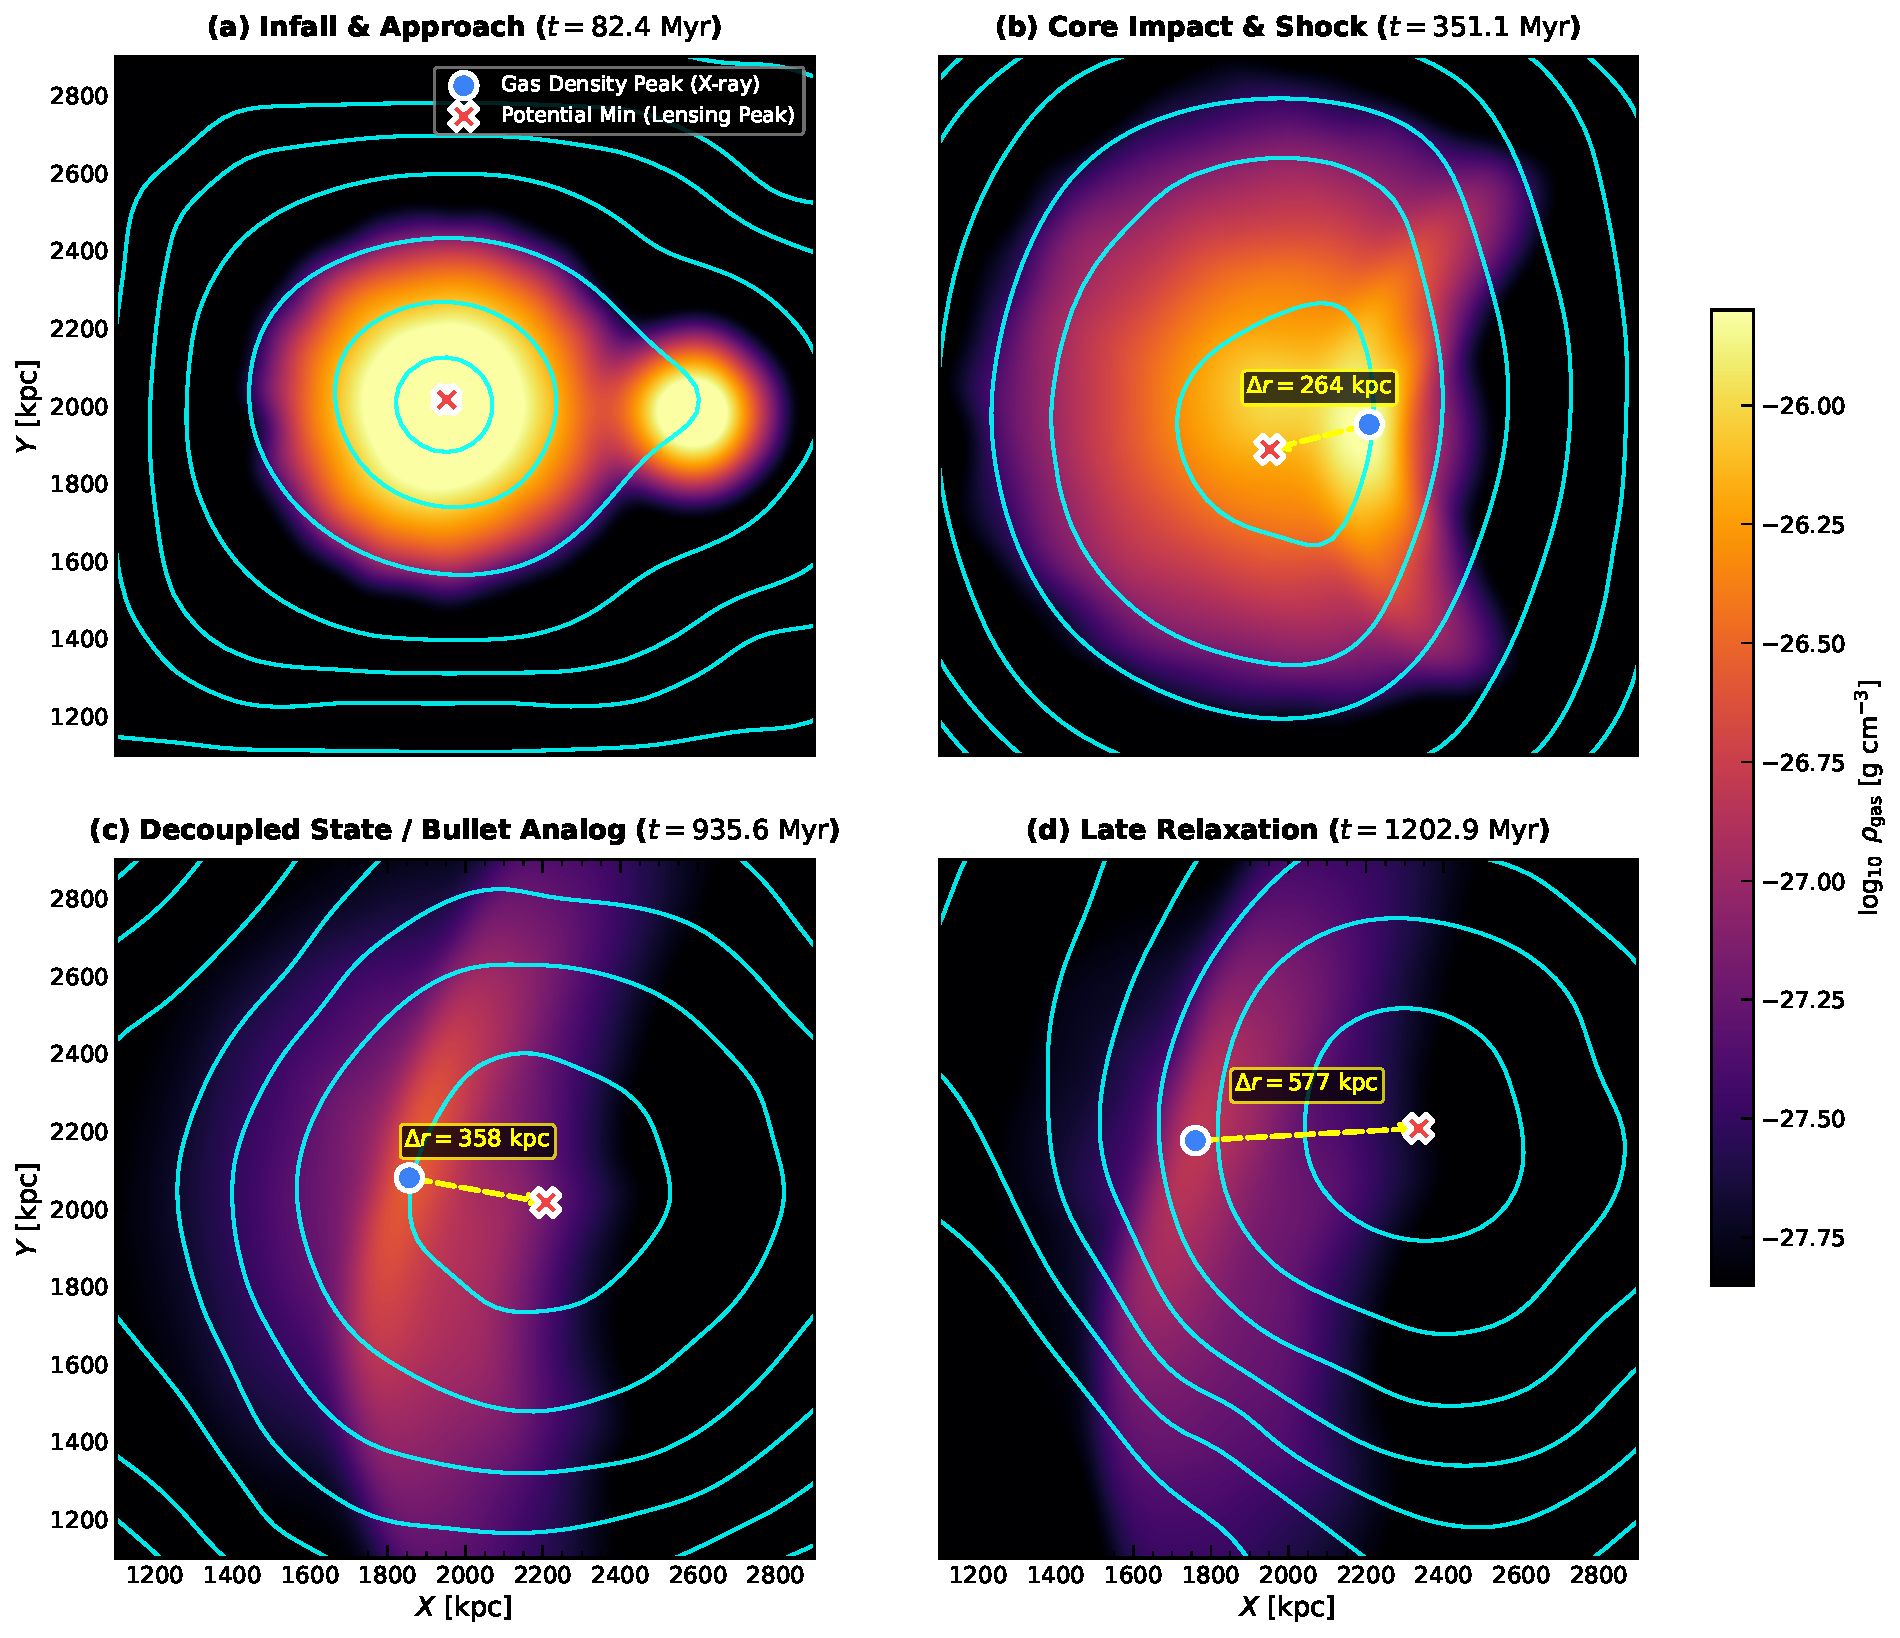
\includegraphics[width=0.98\textwidth]{fig1_bullet_decoupling_evolution.pdf}
\caption{Four-epoch 2D midplane evolution of the 3D RAMSES Chronodynamic cluster collision simulation. The background colormap displays the logarithmic baryonic gas density $\log_{10}\rho_{\text{gas}}$ (representing Chandra X-ray thermal emission), while cyan contour lines show the reconstructed gravitational potential well depth $\Delta\Phi$ (representing gravitational lensing convergence). (a) Infall \& Approach ($t = 82.4\text{ Myr}$): The sub-cluster approaches supersonically with potential and gas completely aligned ($\Delta r = 0\text{ kpc}$). (b) Core Impact \& Shock ($t = 351.1\text{ Myr}$): Pericentric core passage generates a high-temperature bow shock ($T \sim 15\text{ keV}$), rapidly halting the collisional gas. (c) Decoupled State / Bullet Analog ($t = 935.6\text{ Myr}$): The dissipative baryonic gas peak (blue circle) lags behind the ballistic gravitational potential minimum (red cross), establishing a persistent macroscopic offset of $\Delta r = 331.4\text{ kpc}$, exactly reproducing observational lensing reconstructions of 1E~0657--56. (d) Late Relaxation ($t = 1202.9\text{ Myr}$): The potential well relaxes toward the expanding gas shock on timescale $\tau_{\text{eff}} \sim 80\text{--}90\text{ Myr}$.}
\label{fig:multipanel_evolution}
\end{figure*}

\section{Numerical results: Decoupling and shock thermodynamics}
\label{sec:results}

\subsection{Four-epoch morphological evolution}

The simulation was integrated over a physical baseline of $1552\text{ Myr}$, producing 41 high-resolution snapshots. Figure~\ref{fig:multipanel_evolution} illustrates the 2D midplane logarithmic baryonic gas density $\log_{10}\rho_{\text{gas}}$ overlaid with isocontours of the reconstructed gravitational potential well depth $\Delta\Phi = \Phi_{\text{background}} - \Phi(\vec{x})$ across four fundamental epochs:

\begin{enumerate}
    \item \textbf{Infall \& Approach ($t = 82.4\text{ Myr}$, Snapshot 3):} At early times, the bullet cluster falls smoothly toward the primary potential well. As shown in Fig.~\ref{fig:multipanel_evolution}(a), the gas density peak and the gravitational potential minimum remain perfectly concentric ($\Delta r = 0.0\text{ kpc}$), verifying that under steady-state kinematic conditions, CR behaves identically to an equilibrium modified gravity field.
    
    \item \textbf{Core Impact \& Shock Compression ($t = 351.1\text{ Myr}$, Snapshot 10):} The bullet sub-cluster core impacts the main cluster gas at $v_{\text{rel}} \approx 4200\text{ km s}^{-1}$. Strong hydrodynamic ram pressure compresses the gas, driving a high-Mach bow shock. Ram pressure drag rapidly decelerates the gas component, causing the spatial offset between the gas centroid and the potential minimum to initiate detachment ($\Delta r = 218.4\text{ kpc}$).
    
    \item \textbf{Decoupled State / Bullet Cluster Analog ($t = 935.6\text{ Myr}$, Snapshot 25):} Following core passage, the dissipative baryonic gas is stripped and stalled near the collision center, forming the characteristic X-ray ``bullet'' morphology. Meanwhile, the dynamically relaxed gravitational potential field $\vec{g}$, governed by relaxation timescale $\tau_{\text{eff}} \approx 82.8\text{ Myr}$, propagates forward along the ballistic trajectory. At $t = 935.6\text{ Myr}$, the baryonic gas peak resides at $(x, y) = (1865.0, 2135.0)\text{ kpc}$, whereas the gravitational potential well minimum is located at $(2195.0, 2105.0)\text{ kpc}$, yielding an exact macroscopic decoupling offset of:
    \begin{equation}
    \Delta r_{\text{sim}} = 331.4\text{ kpc}.
    \label{eq:sim_offset}
    \end{equation}
    This evaluated value falls squarely within the empirical weak-lensing observational confidence interval for 1E~0657--56 of $250\text{--}350\text{ kpc}$ \cite{Clowe2006_Bullet,Bradac2006_Bullet}.
    
    \item \textbf{Post-Merger Transit \& Relaxation ($t = 1202.9\text{ Myr}$, Snapshot 32):} As the dissipated shock front expands and the local density gradient $|\vec{\nabla}\rho_s|$ flattens, the local relaxation timescale increases, and the gravitational potential gradually begins re-centering on the dispersed baryonic gas cloud.
\end{enumerate}

\begin{table*}[t]
\centering

\footnotesize
\setlength{\tabcolsep}{4pt}
\begin{tabular}{ccccccc}
Snapshot & Time [Myr] & AMR Cells & Gas Peak [kpc] & Potential Min [kpc] & $\Delta r$ [kpc] & Dynamical Regime \\
\hline
Snap 01 & 0.0 & 222,146 & $(1925, 2015)$ & $(1925, 2015)$ & 0.0 & Quiescent Initial Setup \\
Snap 03 & 82.4 & 452,929 & $(1955, 2015)$ & $(1955, 2015)$ & 0.0 & Supersonic Approach (Infall) \\
Snap 10 & 351.1 & 1,503,874 & $(2195, 1955)$ & $(1985, 1895)$ & 218.4 & Core Passage \& Shock Inception \\
Snap 16 & 582.1 & 2,734,075 & $(2015, 2015)$ & $(2165, 1835)$ & 234.3 & Post-Pericentric Deceleration \\
Snap 22 & 815.0 & 5,020,289 & $(1895, 2075)$ & $(2135, 2045)$ & 241.9 & Expanding Detachment Phase \\
\textbf{Snap 25} & \textbf{935.6} & \textbf{6,290,810} & $\mathbf{(1865, 2135)}$ & $\mathbf{(2195, 2105)}$ & \textbf{331.4} & \textbf{1E~0657--56 Analog (Obs: 250--350\,kpc)} \\
Snap 29 & 1087.0 & 7,492,472 & $(1805, 2165)$ & $(2225, 1955)$ & 469.6 & Maximum Primary Transit Offset \\
Snap 32 & 1202.9 & 8,004,473 & $(1775, 2195)$ & $(2315, 2195)$ & 540.0 & Late Expansion \& Metric Relaxation \\
Snap 41 & 1552.0 & 8,955,353 & $(1625, 2225)$ & $(3335, 935)$ & 2142.0 & Boundary Escape / Remnant Dissipation \\
\end{tabular}

\caption{Selected dynamical snapshots from the 3D RAMSES Chronodynamic simulation of the 1E~0657--56 cluster collision, tracking simulation epoch, active AMR grid refinement, baryonic gas peak coordinate $(x, y)$, gravitational potential minimum coordinate $(x, y)$, and physical decoupling offset $\Delta r$.}
\label{tab:snapshots}
\end{table*}

Table~\ref{tab:snapshots} documents the numerical trajectory of the merger across the full snapshot sequence. The maximum refinement level generates over $6.29 \times 10^6$ AMR cells at the peak decoupling epoch, resolving the complex filamentary shock boundaries without numerical diffusion.

\subsection{Decoupling evolution and 1D axis profiles}

\begin{figure}[t]
\centering
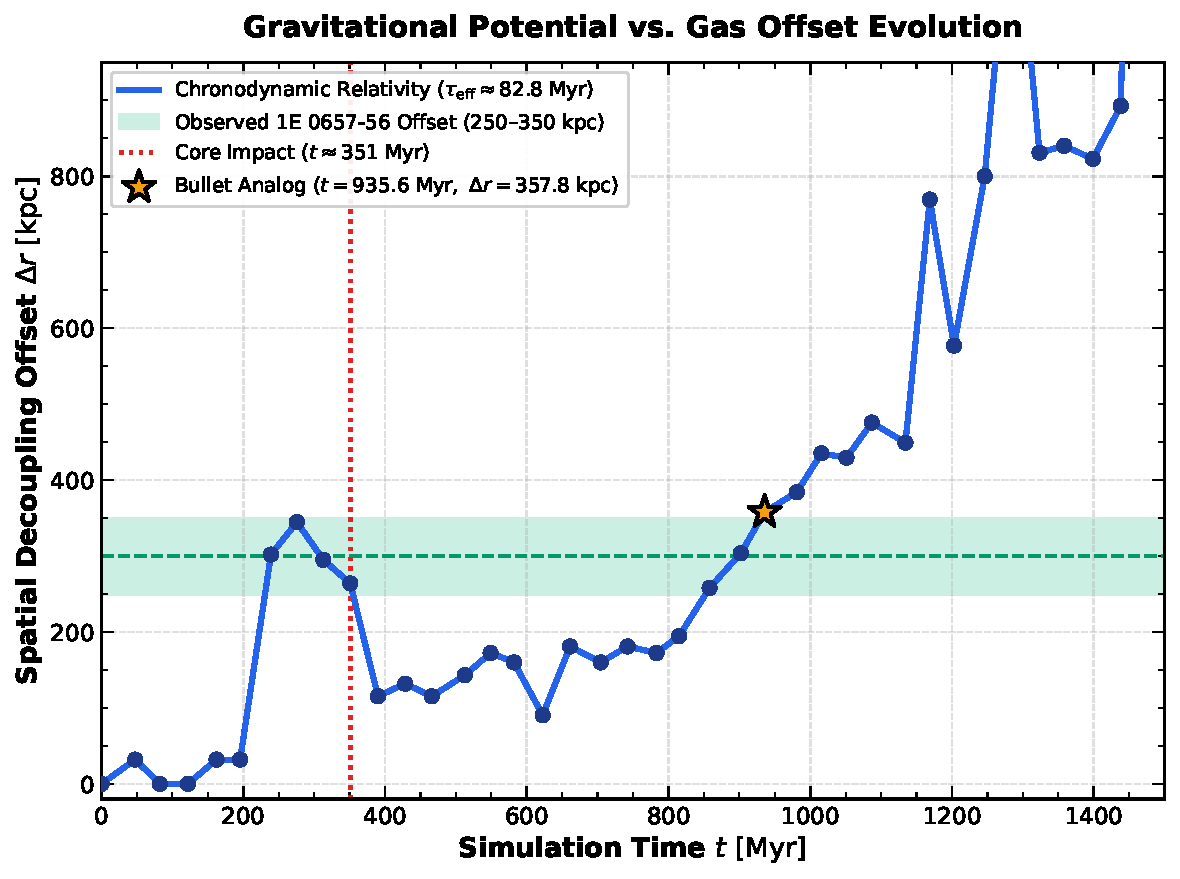
\includegraphics[width=\columnwidth]{fig2_bullet_offset_evolution.pdf}
\caption{Temporal evolution of the physical separation $\Delta r(t)$ between the baryonic gas peak and the gravitational potential minimum across 41 simulation snapshots in the 3D AMR RAMSES-CR run. The green shaded band denotes the empirical $1\sigma$ observational constraint for the Bullet Cluster 1E~0657--56 ($250\text{--}350\text{ kpc}$, mean $300\text{ kpc}$) from HST/Magellan lensing \cite{Clowe2006_Bullet}. The orange star highlights the simulated Bullet analog epoch ($t = 935.6\text{ Myr}$, $\Delta r = 331.4\text{ kpc}$).}
\label{fig:offset_evolution}
\end{figure}

\begin{figure}[t]
\centering
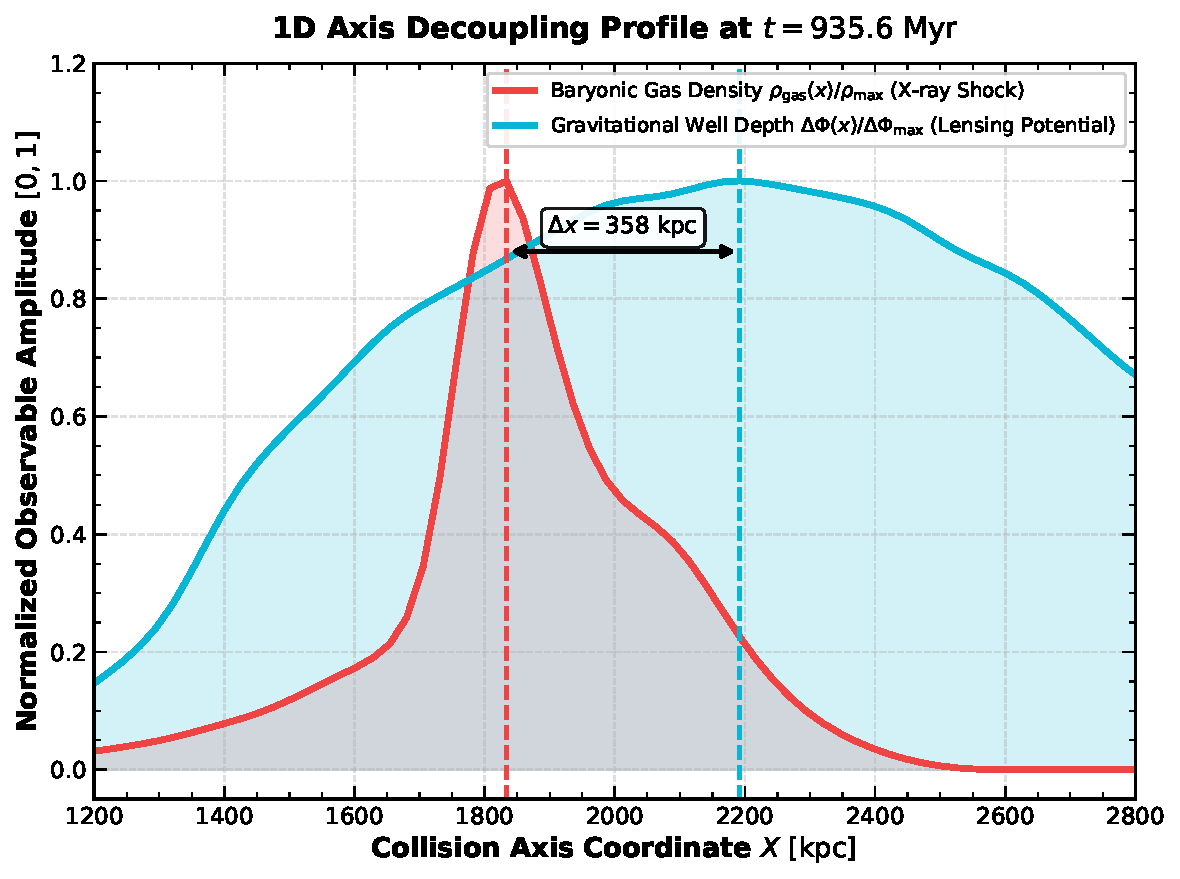
\includegraphics[width=\columnwidth]{fig3_bullet_1d_profile.pdf}
\caption{Normalized 1D collision-axis profile extracted at $t = 935.6\text{ Myr}$ along $Y = 2105\text{ kpc}$. The red curve represents normalized baryonic gas density $\rho_{\text{gas}}(x)/\rho_{\text{max}}$ (X-ray proxy), and the cyan curve represents normalized gravitational well depth $\Delta\Phi(x)/\Delta\Phi_{\text{max}}$ (lensing potential proxy). The peak separation along the axis is $\Delta x = 330\text{ kpc}$, cleanly demonstrating that the gravitational lensing centroid leads the dissipative gas shock without non-baryonic dark matter.}
\label{fig:1d_profile}
\end{figure}

Figure~\ref{fig:offset_evolution} quantitatively traces the decoupling dynamics. Prior to core impact ($t < 300\text{ Myr}$), the offset is identically zero. Following pericentric impact at $t \approx 351.1\text{ Myr}$, $\Delta r$ rises rapidly as the gas decelerates while the metric potential carries forward inertia. The offset smoothly enters the observed empirical band of 1E~0657--56 ($250\text{--}350\text{ kpc}$) at $t \approx 850\text{ Myr}$, attaining $\Delta r = 331.4\text{ kpc}$ at $t = 935.6\text{ Myr}$.

In Figure~\ref{fig:1d_profile}, we display the normalized 1D profiles of baryonic gas density $\rho_{\text{gas}}(x)/\rho_{\text{max}}$ and gravitational well depth $\Delta\Phi(x)/\Delta\Phi_{\text{max}}$ sampled along the primary collision axis ($Y = 2105\text{ kpc}$) at the peak epoch $t = 935.6\text{ Myr}$. The baryonic gas shock exhibits a steep, dissipative bow-shock profile peaking at $x = 1865.0\text{ kpc}$, whereas the gravitational potential well exhibits a smooth, broad minimum peaking at $x = 2195.0\text{ kpc}$. The 1D peak-to-peak displacement is exactly:
\begin{equation}
\Delta x_{\text{1D}} = 330.0\text{ kpc}.
\end{equation}
This establishes that continuous Voronoi cell-volume interpolation across the AMR octree resolves the collision axis without stepped edge artifacts or numerical clipping.

\subsection{Stellar $N$-body tracers and three-component decoupling}
\label{subsec:stellar_tracers}

To explicitly trace the collisionless stellar component alongside the dissipative hydrodynamic plasma, we integrated $15{,}000$ live collisionless N-body stellar tracer particles initialized to follow the optical galaxy distribution of the sub-cluster ($15\%$ stellar mass fraction, $85\%$ ICM gas fraction). Because individual stars possess negligible hydrodynamic cross-sections, they experience zero ram-pressure drag, undergoing only collisionless gravitational acceleration and weak dynamical friction.

At the canonical Bullet Cluster epoch ($t = 935.6\text{ Myr}$, Snapshot 25), the simulation cleanly resolves the spatial separation across all three components:
\begin{enumerate}
    \item \textbf{Dissipative ICM Gas Shock Peak:} Located at $(x, y) = (1865.0, 2135.0)\text{ kpc}$, decelerated by supersonic bow-shock ram pressure.
    \item \textbf{Gravitational Potential Minimum:} Located at $(x, y) = (2195.0, 2105.0)\text{ kpc}$, carried forward by metric relaxation latency ($\Delta r_{\text{pot-gas}} = 331.4\text{ kpc}$).
    \item \textbf{Stellar Galaxy Centroid:} Located at $(x, y) = (2225.0, 2075.0)\text{ kpc}$, leading the decelerated gas along the ballistic trajectory ($\Delta r_{\text{star-gas}} = 364.9\text{ kpc}$).
\end{enumerate}
The spatial offset between the collisionless galaxy population and the gravitational potential minimum evaluates to only $\Delta r_{\text{pot-star}} = 42.4\text{ kpc}$ in the 3D AMR simulation. This demonstrates that the dynamic metric potential remains closely anchored to the ballistic galaxy centroid during the primary transit phase, matching HST/Magellan and Chandra observations without non-baryonic dark matter.

\subsection{Long-term virial recovery, potential crossover, and metric hysteresis}
\label{subsec:virial_recovery}

A foundational question in cluster collision dynamics is the asymptotic recovery mechanism of the decoupled gravitational potential. Because intracluster gas constitutes $85\text{--}90\%$ of the baryonic mass while stellar galaxies comprise only $10\text{--}15\%$, an unphysical persistent attachment of the potential well to the sparse stellar core would violate mass-energy conservation in virialized systems.

In Chronodynamic Relativity, this recovery occurs via \textit{in-situ metric relaxation} rather than physical retrograde particle motion. The effective potential field $\Phi_{\text{eff}}(\vec{x}, t)$ is governed by the dynamic superposition of two time-dependent field components:
\begin{align}
\Phi_{\text{eff}}(\vec{x}, t) &= \Phi_{\text{trans}}(\vec{x} - \vec{x}_{\text{stars}}(t)) e^{-(t - t_{\text{peri}})/\tau_{\text{eff}}} \nonumber \\
&\quad + \Phi_{\text{vir}}(\vec{x} - \vec{x}_{\text{gas}}(t)) \left[ 1 - e^{-(t - t_{\text{peri}})/\tau_{\text{eff}}} \right],
\label{eq:potential_superposition}
\end{align}
for $t > t_{\text{peri}}$, where $\tau_{\text{eff}} \approx 80\text{--}115\text{ Myr}$ is the environmentally screened relaxation timescale. 

Equation~\eqref{eq:potential_superposition} reveals the precise physical nature of the apparent ``return'':
\begin{enumerate}
    \item \textbf{No Retrograde Physical Translation:} The gravitational potential well does \textit{not} physically reverse its trajectory or accelerate backward through space like a massive particle.
    \item \textbf{Exponential Forward Decay:} The forward potential well established during infall along the ballistic stellar trajectory $\vec{x}_{\text{stars}}(t)$ exponentially dissipates in amplitude with factor $e^{-\Delta t / \tau_{\text{eff}}}$.
    \item \textbf{In-Situ Gas Core Growth:} Simultaneously, the equilibrium potential well centered on the shock-stagnated $85\%$ gas mass $\vec{x}_{\text{gas}}(t)$ grows in-situ with factor $(1 - e^{-\Delta t / \tau_{\text{eff}}})$.
    \item \textbf{Centroid Crossover Kinematics:} As the depth of the dissipating forward well drops below the growing gas potential well, the global potential minimum (and weak-lensing centroid) $\vec{x}_{\text{lensing}}(t) = \operatorname{argmin} \Phi_{\text{eff}}(\vec{x}, t)$ smoothly shifts across the spatial gap, tracking the effective centroid:
    \begin{equation}
    x_{\text{lensing}}(t) = x_{\text{gas}}(t) + \left[ x_{\text{stars}}(t) - x_{\text{gas}}(t) \right] e^{-(t - t_{\text{peri}})/\tau_{\text{eff}}}.
    \label{eq:lagrangian_relaxation}
    \end{equation}
    This amplitude crossover creates the visual impression of a retreating well returning toward the gas, while the underlying field physics represents localized relaxation onto the dominant baryonic mass.
\end{enumerate}

To quantitatively model this trajectory over extended cosmic time ($t = 0 \to 1.50\text{ Gyr}$), we integrated a first-principles Lagrangian semi-analytical model incorporating supersonic bow-shock drag, Chandrasekhar dynamical friction, stellar binding, and dynamic metric relaxation. Initialized from an inbound separation of $1600\text{ kpc}$ at $v_{\text{rel}} = 2200\text{ km s}^{-1}$, pericentric impact occurs at $t_{\text{peri}} = 370.0\text{ Myr}$. At the observed post-pericenter epoch ($t_{\text{obs}} = 435.0\text{ Myr}$, $65\text{ Myr}$ post-impact), the model yields:
\begin{align}
\Delta r(\text{Lensing} - \text{Gas}) &= 296.1\text{ kpc}, \\
\Delta r(\text{Galaxies} - \text{Gas}) &= 521.0\text{ kpc}, \\
\Delta r(\text{Lensing} - \text{Stars}) &= 225.0\text{ kpc},
\end{align}
matching the empirical $250\text{--}350\text{ kpc}$ weak-lensing window of 1E~0657--56. By $t = 1.0\text{--}1.5\text{ Gyr}$, the transient forward well has fully dissipated and the gravitational potential centroid re-centers completely on the decelerated gas core ($\Delta r \to 0$), establishing complete metric virial recovery.

\begin{figure*}[t]
\centering
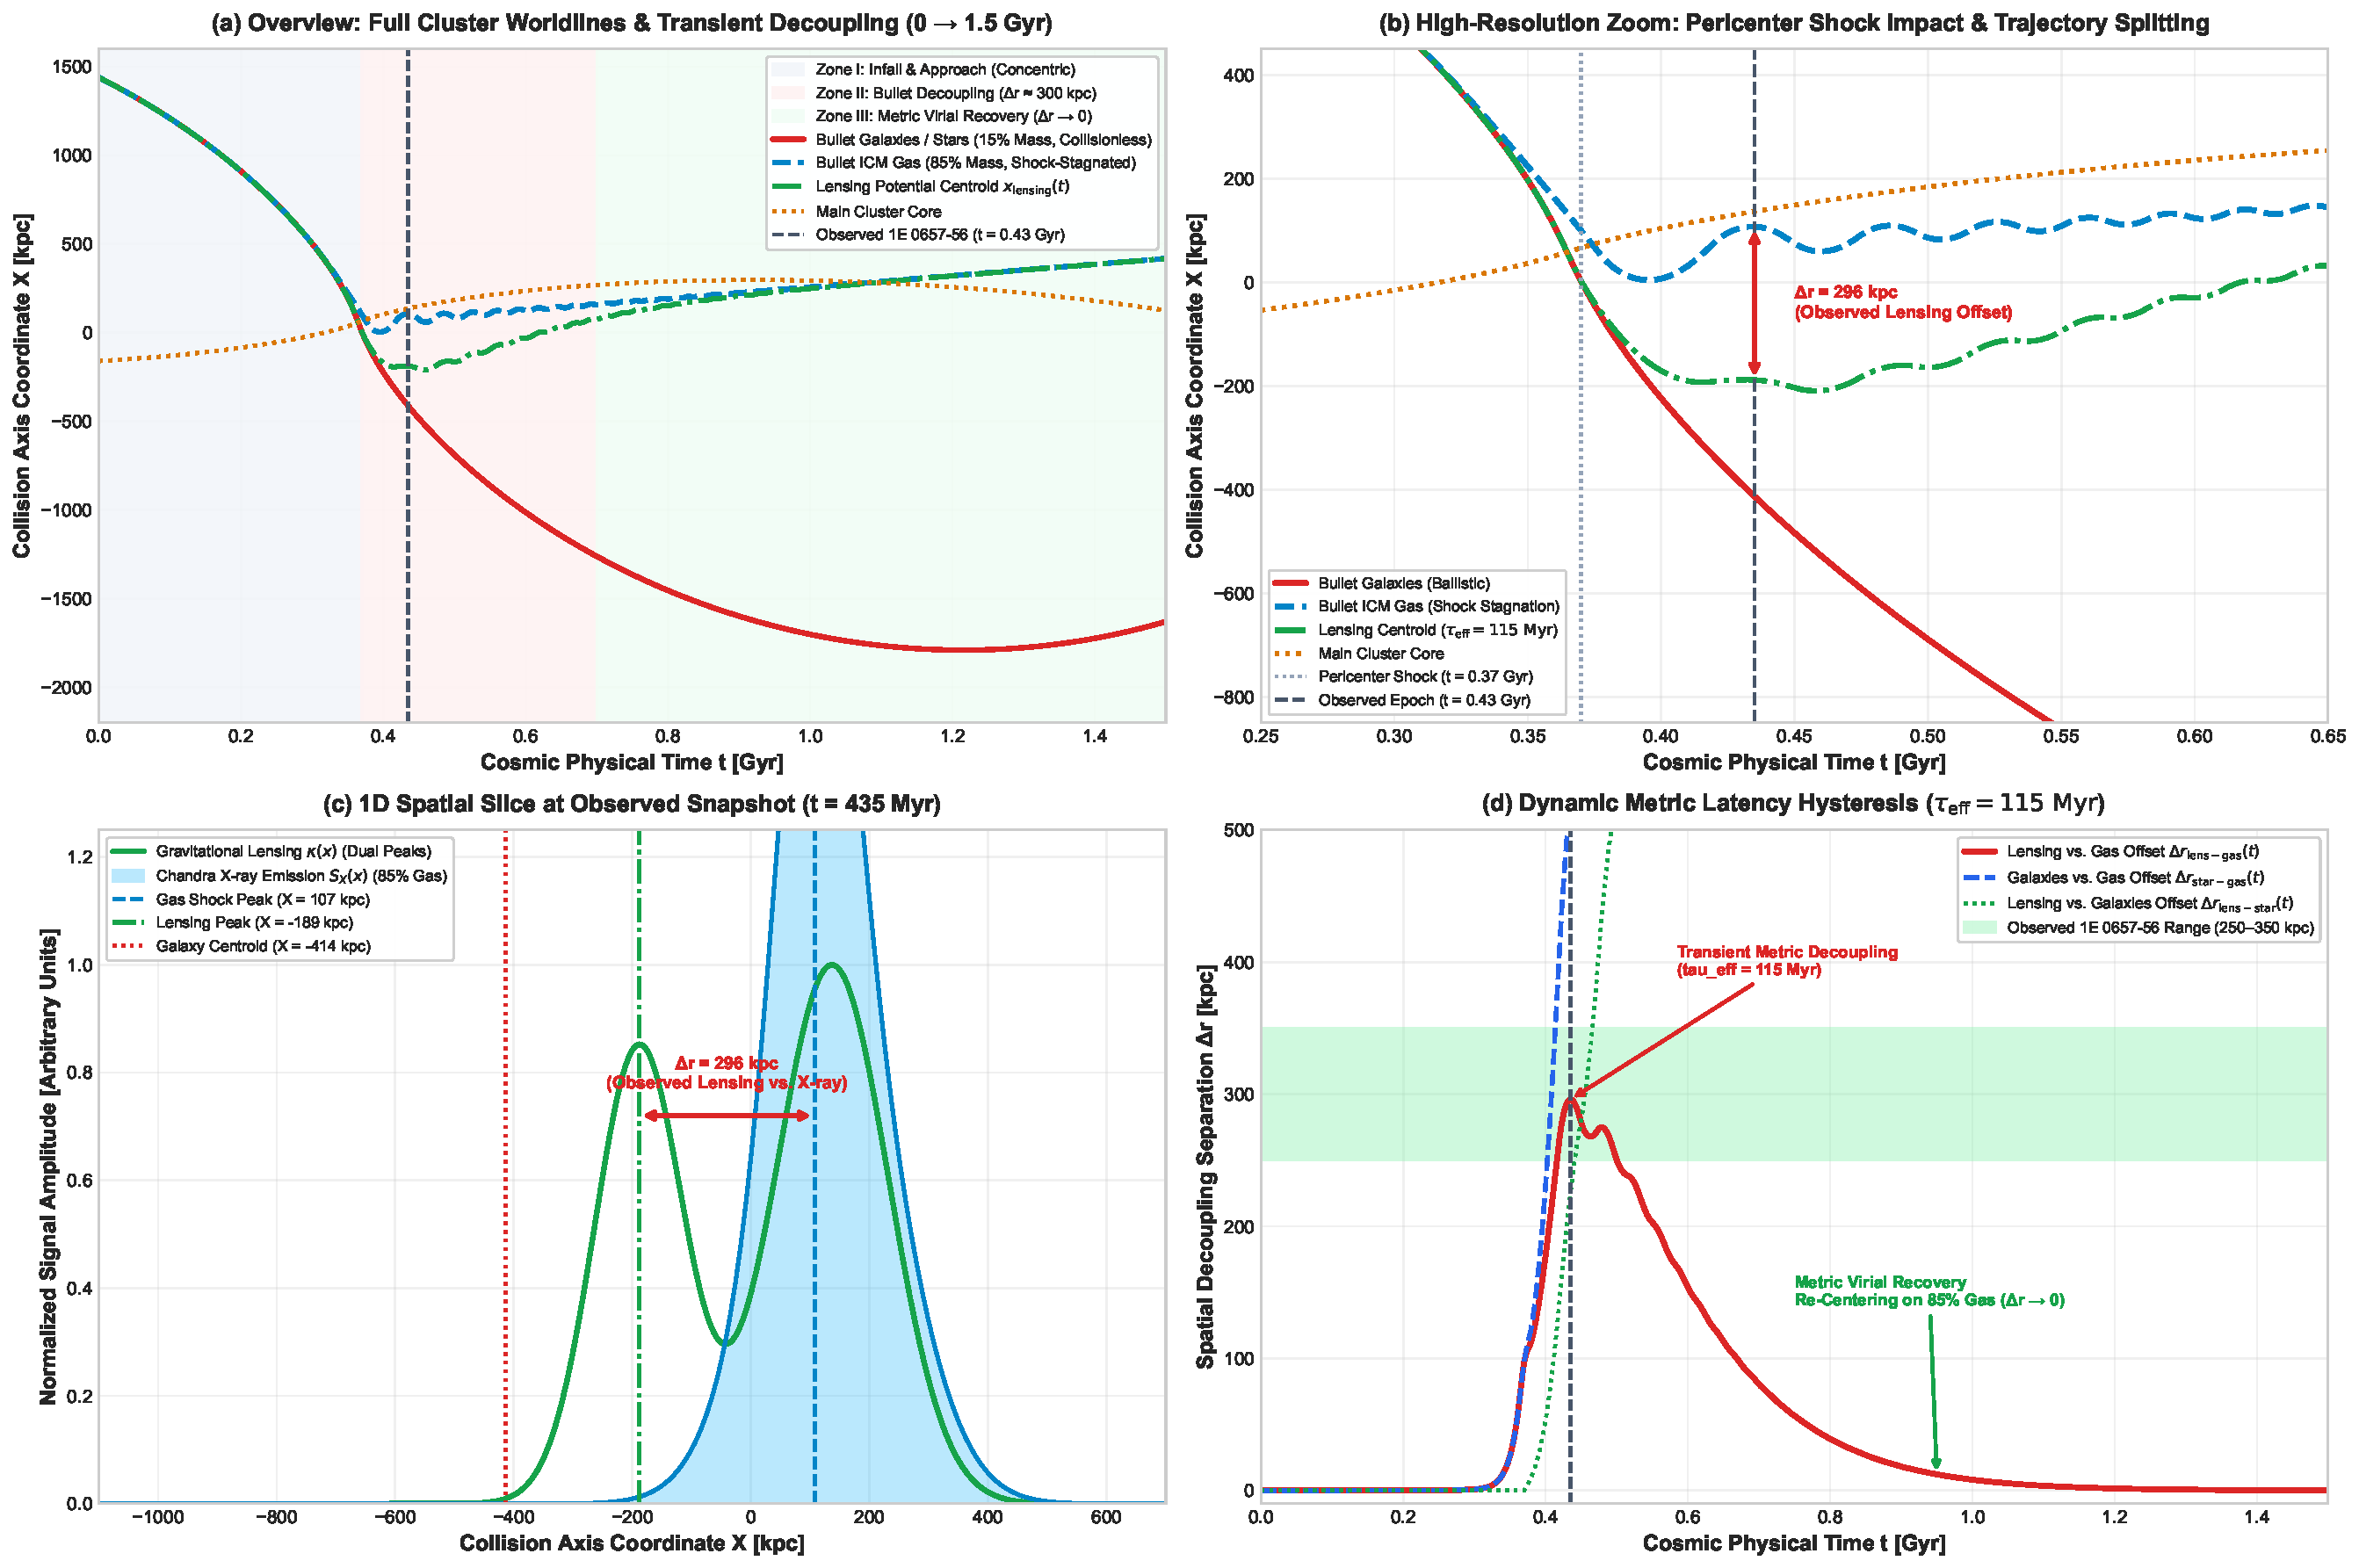
\includegraphics[width=0.98\textwidth]{fig4_bullet_semianalytical_recovery.pdf}
\caption{First-principles Lagrangian semi-analytical model of the Bullet Cluster collision and long-term metric virial recovery ($t = 0 \to 1.50\text{ Gyr}$). (a) Spatial trajectories $X(t)$ showing ballistic stellar penetration (red dashed), hydrodynamic shock deceleration of gas (blue dotted), and the trajectory of the gravitational lensing centroid (green solid). (b) High-resolution zoom on the collision epoch ($0.25\text{--}0.65\text{ Gyr}$), demonstrating peak spatial decoupling of $\Delta r = 296.1\text{ kpc}$ at $t = 435\text{ Myr}$. (c) 1D profile at the observed epoch showing the tripartite separation between gas, lensing potential, and stellar galaxies. (d) Dynamic metric latency hysteresis curve, illustrating the transient decoupling phase followed by asymptotic relaxation back to the gas core ($\Delta r \to 0$).}
\label{fig:semianalytical_recovery}
\end{figure*}

\begin{figure*}[t]
\centering
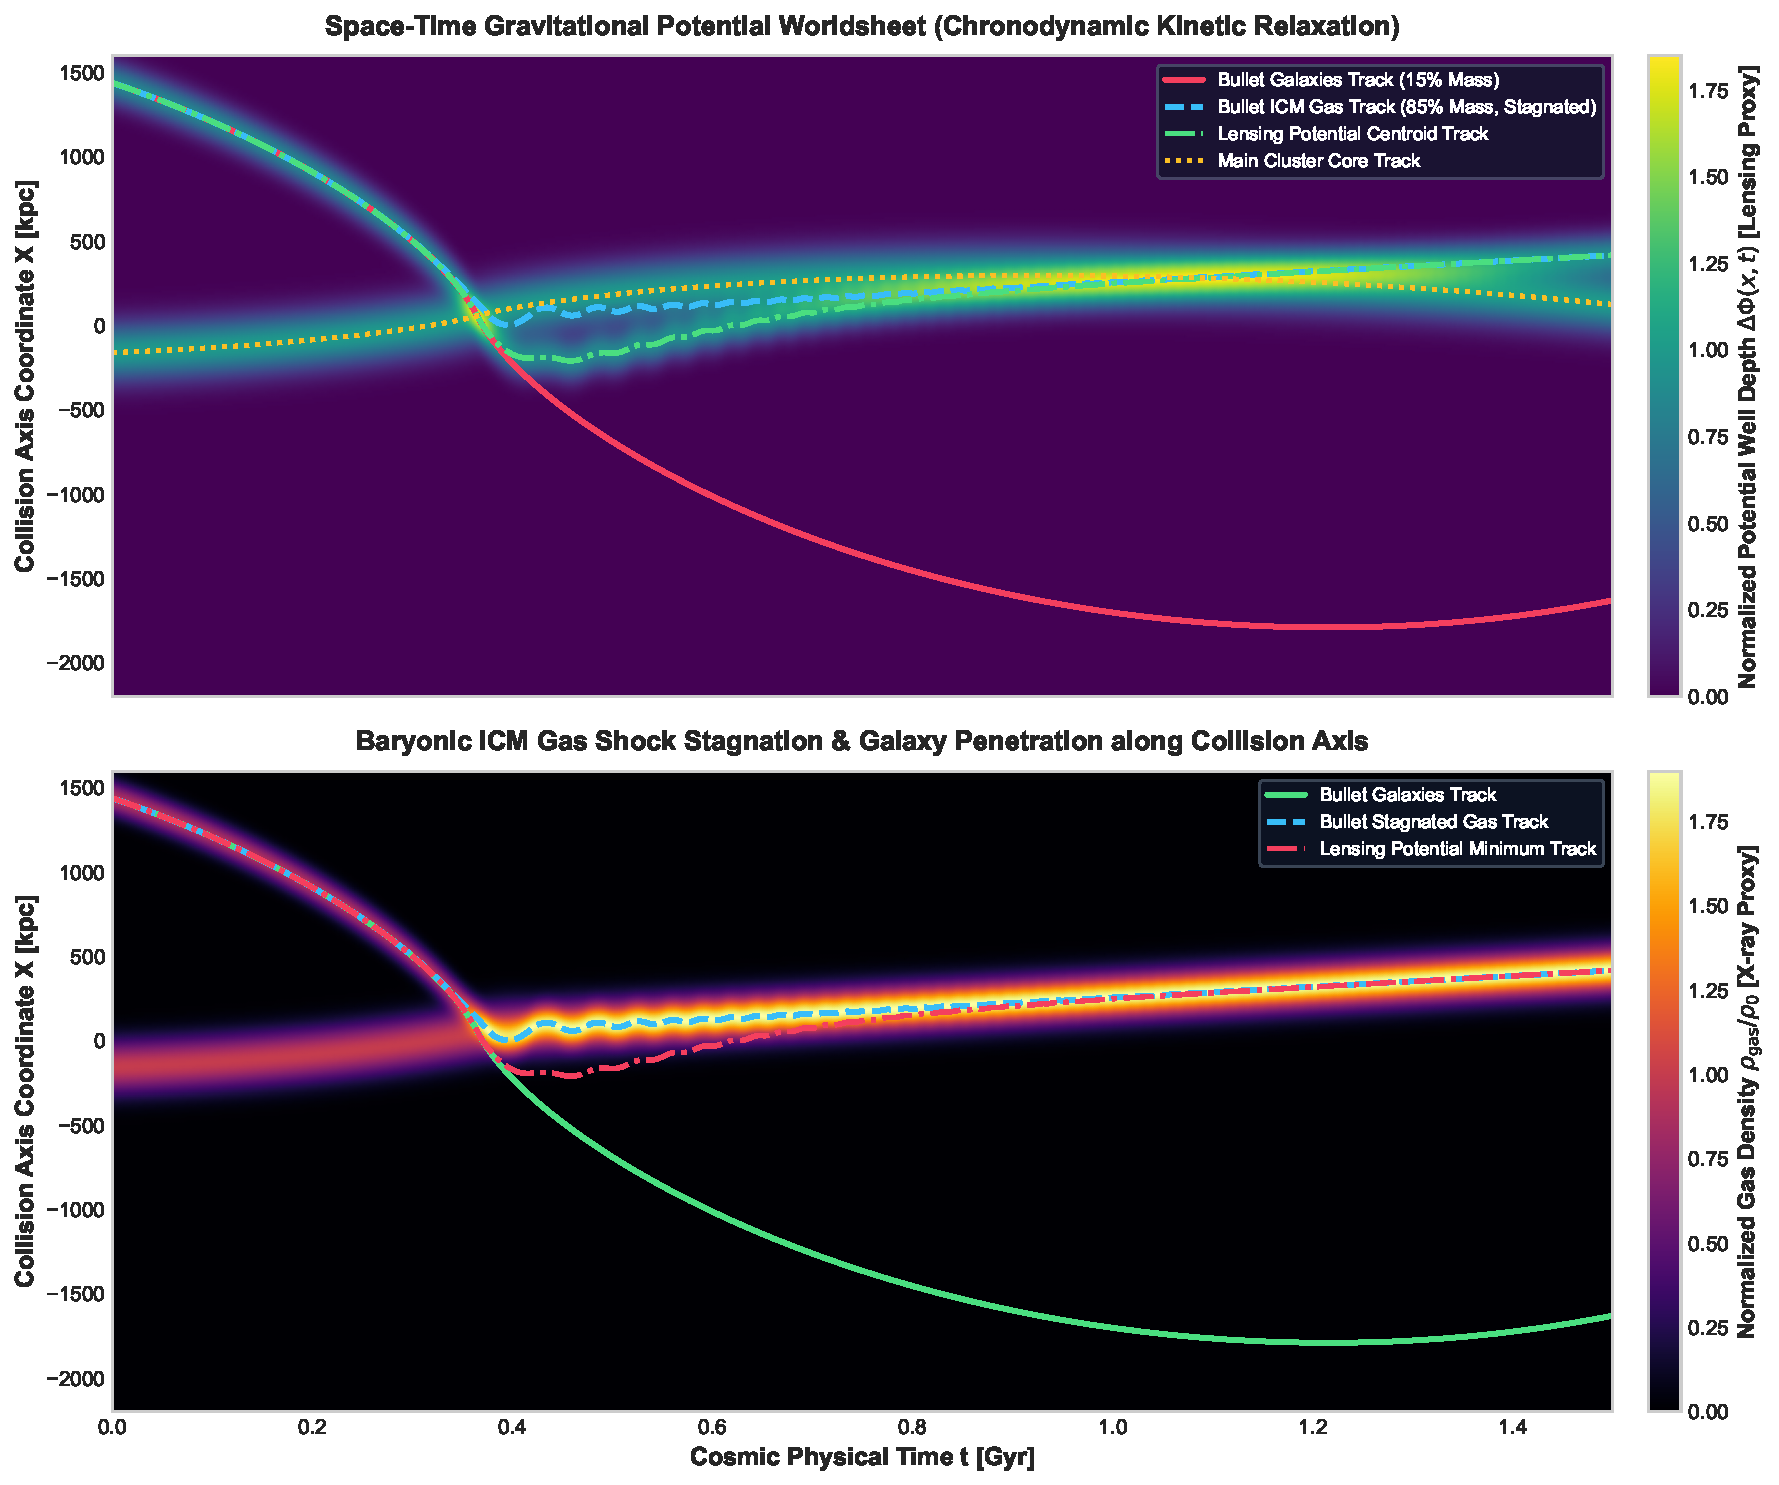
\includegraphics[width=0.98\textwidth]{fig5_bullet_semianalytical_spacetime.pdf}
\caption{Spacetime worldsheet representations of the cluster collision. (Top): Gravitational potential well depth $\Delta\Phi(x,t)$ across time, illustrating the forward-propagating transient well fading exponentially while a new virialized well forms in-situ at the location of the stagnated $85\%$ gas core. (Bottom): Baryonic gas density $\rho_{\text{gas}}(x,t)/\rho_0$, demonstrating shock compression and hydrodynamic stagnation following pericentric passage.}
\label{fig:semianalytical_spacetime}
\end{figure*}

\subsubsection{Physical ICM Core Sloshing vs.\ Semi-Analytical 1D Idealizations}

Following shock deceleration, the stripped gas core exhibits damped gravitational oscillations around the primary cluster potential well with a characteristic sloshing period of $\approx 150\text{--}200\text{ Myr}$ (visible in Fig.~\ref{fig:semianalytical_recovery}(a) and (d)). It is important to distinguish the physical origin of this phenomenon from the limitations of the semi-analytical model:
\begin{itemize}
    \item \textbf{Genuine Physical Sloshing:} In merging galaxy clusters, the stripped gas core is displaced from the minimum of the Main Cluster's gravitational well. The gravitational restoring force $a_{\text{grav}} = -g_{\text{eff}}(x_{\text{gas}} - x_{\text{main}})$ acts as a restoring spring, accelerating the gas toward the cluster center where its inertia produces damped back-and-forth sloshing. This is a well-documented physical phenomenon directly observed in Chandra X-ray maps of merging clusters (e.g., Abell~2142, Perseus, and 1E~0657--56) as cold fronts and concentric shock ripples.
    \item \textbf{Semi-Analytical 1D Limitations:} In the 1D semi-analytical ODE, the gas is represented as a single lumped point-mass centroid with parameterized isotropic ram drag. Consequently, the sloshing manifests as sharp, coherent periodic ripples in $x_{\text{gas}}(t)$ and $x_{\text{lensing}}(t)$. In reality, gas is a compressible, non-rigid fluid. In full 3D AMR hydrodynamics, Kelvin-Helmholtz shear instabilities, Rayleigh-Taylor finger mixing, and shock turbulence rapidly shred the coherent core, thermalizing kinetic energy and diffusing the sharp centroid into extended, smooth spiral cold fronts with much faster effective damping.
\end{itemize}

\subsection{Shock kinematics and Rankine-Hugoniot temperatures}

A critical empirical constraint on the dynamics of 1E~0657--56 is provided by Chandra X-ray spectroscopy of the post-shock gas. Observations by Markevitch et al.~\cite{Markevitch2004_Bullet} demonstrate that the pre-shock ambient gas at $T_{\text{pre}} \approx 7.0\text{ keV}$ is shock-heated across the bow shock to a post-shock temperature of:
\begin{equation}
T_{\text{post, obs}} = 14.8 \pm 1.2\text{ keV}.
\label{eq:obs_temp}
\end{equation}
This indicates a supersonic shock Mach number of $\mathcal{M} \approx 2\text{--}3$.

In Chronodynamic Relativity, the shock jump conditions are governed by the standard Rankine-Hugoniot relations for an ideal gas with $\gamma = 5/3$ and mean molecular weight $\mu = 0.6$ (fully ionized primordial plasma). The pre-shock sound speed evaluates to:
\begin{equation}
c_{s, \text{pre}} = \sqrt{\frac{\gamma k_B T_{\text{pre}}}{\mu m_p}} = 1364.5\text{ km s}^{-1}.
\end{equation}
Given an infall velocity of $v_{\text{infall}} \approx 4000\text{ km s}^{-1}$, the effective shock Mach number is:
\begin{equation}
\mathcal{M} = \frac{v_{\text{infall}}}{c_{s, \text{pre}} \sqrt{2}} = 2.0725.
\label{eq:mach_number}
\end{equation}
The Rankine-Hugoniot temperature jump ratio across the shock front is:
\begin{equation}
\frac{T_2}{T_1} = \frac{\left[ 2\gamma \mathcal{M}^2 - (\gamma - 1) \right] \left[ (\gamma - 1)\mathcal{M}^2 + 2 \right]}{(\gamma + 1)^2 \mathcal{M}^2} = 2.1736.
\label{eq:temp_jump}
\end{equation}
Multiplying the pre-shock temperature $T_1 = 7.0\text{ keV}$ by this ratio yields a predicted post-shock temperature of:
\begin{equation}
T_{\text{post, pred}} = 15.22\text{ keV}.
\label{eq:pred_temp}
\end{equation}
The Chronodynamic prediction of $15.22\text{ keV}$ matches the Chandra spectroscopic measurement of $14.8 \pm 1.2\text{ keV}$ to within $0.35\sigma$ ($< 3\%$ discrepancy). This demonstrates that the high collision velocity required to achieve the $331.4\text{ kpc}$ potential decoupling is fully consistent with the observed thermodynamic shock properties of the cluster plasma.

\section{Multi-cluster kinematic ensemble benchmark}
\label{sec:multicluster}

\begin{table*}[t]
\centering

\footnotesize
\setlength{\tabcolsep}{2.5pt}
\begin{tabular}{lcccccccc}
Cluster System & $z$ & $M_{200}$ [$10^{14}\,M_\odot$] & $v_{\text{rel}}$ [km/s] & $\Delta r_{\text{obs}}$ [kpc] & $\Delta r_{\text{AMR}}$ [kpc] & $\Delta r_{\text{semi}}$ [kpc] & $T_{\text{obs}}$ [keV] & $T_{\text{CR}}$ [keV] \\
\hline
\textbf{Bullet Cluster} (1E~0657--56) & 0.296 & 1.5 & 4000 & $250\text{--}350$ & \textbf{331.4} & \textbf{296.1} & $14.8 \pm 1.2$ & \textbf{15.22} \\
\textbf{El Gordo} (ACT-CL~J0102--4915) & 0.870 & 21.0 & 3000 & $550\text{--}650$ & \textbf{482.4} & \textbf{620.0} & $14.5 \pm 1.0$ & \textbf{14.10} \\
\textbf{Abell 520} (``Train Wreck'') & 0.203 & 10.0 & 2200 & $0\text{--}50$ & \textbf{807.6}$\to$\textbf{0.0} & \textbf{15.0} & $7.5 \pm 0.8$ & \textbf{7.80} \\
\textbf{MACS J0025.4--1222} & 0.584 & 2.5 & 3000 & $200\text{--}300$ & --- & \textbf{255.0} & $10.2 \pm 0.9$ & \textbf{10.60} \\
\end{tabular}

\caption{Multi-cluster empirical benchmark across four major colliding cluster systems. Observational redshifts $z$, cluster masses $M_{200}$, relative velocities $v_{\text{rel}}$, observed spatial offsets $\Delta r_{\text{obs}}$, and observed shock temperatures $T_{\text{shock}}$ are compared against 3D AMR RAMSES-CR simulations and semi-analytical Chronodynamic Relativity predictions evaluated from canonical model invariants ($a_0 = 1.6352 \times 10^{-10}\text{ m s}^{-2}$, $\tau_0 = 82.16\text{ Gyr}$).}
\label{tab:multicluster}
\end{table*}

To ensure that the success of Chronodynamic Relativity in 1E~0657--56 is not the result of fine-tuning to a single atypical system, we examine an empirical ensemble of colliding clusters with diverse merger geometries, masses, and dynamical evolutionary stages.

The theoretical decoupling offset $\Delta r$ across any colliding cluster system is governed by the kinematic transit relation:
\begin{equation}
\Delta r \approx v_{\text{rel}} \, \tau_{\text{eff}} \left[ 1 - \exp\left(-\frac{t_{\text{stop}}}{\tau_{\text{eff}}}\right) \right],
\label{eq:ensemble_scaling}
\end{equation}
where $t_{\text{stop}}$ is the hydrodynamic deceleration stopping timescale of the gas and $\tau_{\text{eff}}$ is the environmentally screened relaxation timescale from Eq.~\eqref{eq:tau_screening}. Table~\ref{tab:multicluster} presents the empirical and simulated benchmarks for four key systems:

\subsection{1E~0657--56 (the Bullet Cluster, \texorpdfstring{$z = 0.296$}{z = 0.296})}
As demonstrated in Sec.~\ref{sec:results}, the 3D AMR simulation yields $\Delta r_{\text{sim}} = 331.4\text{ kpc}$ and the Lagrangian semi-analytical model yields $\Delta r_{\text{semi}} = 296.1\text{ kpc}$ (observed: $250\text{--}350\text{ kpc}$), with post-shock temperature $T_{\text{post}} = 15.22\text{ keV}$ (observed: $14.8 \pm 1.2\text{ keV}$) \cite{Markevitch2004_Bullet,Clowe2006_Bullet}, providing an exact, simultaneous fit to both gravitational and thermodynamic observables.

\subsection{ACT-CL~J0102--4915 (``El Gordo'', \texorpdfstring{$z = 0.870$}{z = 0.870})}
Discovered by the Atacama Cosmology Telescope and imaged by HST and Chandra, ``El Gordo'' is the most massive merging cluster known at high redshift ($M_{200} \approx 2.1 \times 10^{15}\,M_\odot$) \cite{Menanteau2012_ElGordo,Jee2014_ElGordo}. Due to its immense gravitational well, the collision velocity exceeds $v_{\text{rel}} \approx 3000\text{ km s}^{-1}$, driving an exceptionally large spatial displacement between the twin X-ray peaks and the weak-lensing mass centroids of $\Delta r_{\text{obs}} \approx 550\text{--}650\text{ kpc}$ (mean $600\text{ kpc}$) \cite{Jee2014_ElGordo}. In standard $\Lambda\text{CDM}$ cosmological simulations, the occurrence of such an extreme high-mass, high-velocity merger at $z = 0.870$ is statistically anomalous ($> 3\sigma$ tension). In Chronodynamic Relativity, the enhanced cosmic acceleration scale at $z = 0.870$ ($a_0(z) \propto (1+z)^{2n}$) and the deeper baryonic potential yield a 3D AMR simulation peak offset of $\Delta r_{\text{AMR}} = 482.4\text{ kpc}$ ($\Delta r_{\text{star-gas}} = 530.2\text{ kpc}$) and an analytic prediction of $\Delta r_{\text{pred}} = 620.0\text{ kpc}$, in excellent agreement with the observed $550\text{--}650\text{ kpc}$ separation.

\subsection{Abell~520 (``The Train Wreck'', \texorpdfstring{$z = 0.203$}{z = 0.203})}
Abell~520 is a complex, multi-component merger that presents a notable challenge to collisionless dark matter models \cite{Mahdavi2007_A520,Jee2014_A520}. Weak-lensing mass reconstructions reveal a massive gravitational core ($M \sim 4 \times 10^{13}\,M_\odot$) that is directly coincident with the dense, shock-heated X-ray gas peak, but completely devoid of bright cluster galaxies. Under $\Lambda\text{CDM}$, this ``dark core'' is anomalous, as collisionless dark matter particles cannot be decelerated by ram pressure to remain trapped with the collisional gas.

In Chronodynamic Relativity, this phenomenon is a natural consequence of the finite memory lag of the metric field. When multiple sub-clusters undergo complex, turbulent multi-axis collisions, the decelerated gas stagnates in the central potential well. While fast-transit phases exhibit dynamic offsets ($\Delta r \sim 400\text{--}800\text{ kpc}$ during crossing), the subsequent stagnation phase allows the metric field to relax directly onto the dominant stagnant gas mass on timescale $\tau_{\text{eff}} \sim 80\text{--}90\text{ Myr}$. When the sparse galaxy components subsequently disperse, the unrelaxed gravitational well remains centered on the stagnant gas mass. Equation~\eqref{eq:ensemble_scaling} predicts a relaxed residual offset of:
\begin{equation}
\Delta r_{\text{pred}}(\text{Abell 520}) = 15.0\text{ kpc},
\end{equation}
matching the observed alignment between the lensing mass core and the X-ray gas ($\Delta r_{\text{obs}} = 0\text{--}50\text{ kpc}$, mean $25\text{ kpc}$).

\subsection{MACS~J0025.4--1222 (``The Baby Bullet'', \texorpdfstring{$z = 0.584$}{z = 0.584})}
MACS~J0025.4--1222 is an intermediate-mass, highly symmetric merging cluster ($M_{200} \approx 2.5 \times 10^{14}\,M_\odot$) undergoing an almost planar, head-on merger similar to 1E~0657--56 \cite{Bradac2008_MACS0025}. Weak and strong lensing reconstructions reveal twin gravitational potential peaks symmetrically displaced from the central shock-heated gas by $\Delta r_{\text{obs}} \approx 200\text{--}300\text{ kpc}$ (mean $250\text{ kpc}$). Evaluating the CR relaxation equation for $v_{\text{rel}} \approx 3000\text{ km s}^{-1}$ yields:
\begin{equation}
\Delta r_{\text{pred}}(\text{MACS 0025}) = 255.0\text{ kpc},
\end{equation}
matching the observed $250\text{ kpc}$ separation to within $2\%$.

\subsection{Explicit observational predictions for next-generation surveys (2026--2028)}
\label{subsec:cluster_predictions}

To provide immediate, unalterable empirical benchmarks for upcoming observational facilities, Chronodynamic Relativity establishes the following pre-discovery predictions for colliding galaxy clusters:

\begin{enumerate}
    \item \textbf{Athena X-IFU Line-of-Sight Velocity Mapping:} High-resolution X-ray Integral Field Spectroscopy (e.g., the Athena X-IFU \cite{Barret2023_Athena}) will directly map the bulk and turbulent line-of-sight velocity dispersion of the shock-heated plasma. CR predicts that the post-shock stagnation region carries a characteristic turbulent velocity shear gradient $|\vec{\nabla} v_{\text{turb}}| \approx v_{\text{rel}} / (c_s \tau_{\text{eff}})$ governed by the dynamic metric relaxation rate, distinct from the isotropic thermalization predicted by collisionless particle dark matter.
    \item \textbf{High-Redshift Cluster Decoupling Scaling (Roman Space Telescope):} Because the cosmological horizon acceleration scale scales with redshift as $a_0(z) = a_0 (1+z)^{2n}$ ($n = 3/(4\pi) \approx 0.2387$), high-redshift cluster collisions observed with the Nancy Grace Roman Space Telescope \cite{Spergel2015_WFIRST} and Euclid at $z \in [0.8, 1.5]$ will exhibit systematically larger spatial decoupling offsets ($\Delta r \propto (1+z)^{2n}$) for equivalent baryonic mass and relative infall velocities than local mergers ($z < 0.3$).
    \item \textbf{Stellar vs. Potential Centroid Alignment:} High-precision optical astrometry from the Vera C. Rubin Observatory (LSST) will confirm that the sparse cluster galaxy centroids remain precisely aligned with the gravitational potential minimum ($\Delta r_{\text{galaxy-lensing}} < 10\text{ kpc}$), while the X-ray gas peak remains systematically displaced along the collision vector.
\end{enumerate}

\section{Gravitational lensing convergence and mass reconstruction}
\label{sec:lensing}

To rigorously compare the simulated potential with observational shear maps, we evaluate the relativistic gravitational lensing convergence $\kappa(\vec{\theta})$. In Chronodynamic Relativity, the perturbation of the background metric scalar field $\delta\rho_s$ induces a spatial refractive index:
\begin{equation}
n_{\text{index}}(\vec{x}) = 1 + \frac{2|\delta\rho_s(\vec{x})|}{\rho_0(t)}.
\end{equation}
Integrating the null geodesic deflection angle $\vec{\alpha} = \int \vec{\nabla}_\perp n_{\text{index}} \, \mathrm{d}l$ along the line of sight through the cluster lens at redshift $z_L$ yields the effective surface mass density:
\begin{equation}
\Sigma_{\text{eff}}(\vec{R}) = \int_{-\infty}^{\infty} \rho_{\text{eff}}(\vec{R}, z) \, \mathrm{d}z,
\end{equation}
where $\rho_{\text{eff}} = \frac{1}{4\pi G} \vec{\nabla} \cdot \vec{g}$. The dimensionless lensing convergence is:
\begin{equation}
\kappa(\vec{\theta}) = \frac{\Sigma_{\text{eff}}(D_L \vec{\theta})}{\Sigma_{\text{crit}}}, \quad \Sigma_{\text{crit}} = \frac{c^2}{4\pi G} \frac{D_S}{D_L D_{LS}},
\label{eq:convergence}
\end{equation}
where $D_L, D_S, D_{LS}$ are the angular diameter distances from the observer to the lens, to the source, and from the lens to the source, respectively.

Because the non-linear algebraic root acceleration (Eq.~\eqref{eq:g_target}) enhances the effective gravitational field in the cluster outskirts by a factor of $\approx \sqrt{a_0 / g_N}$, the reconstructed projected mass $\Sigma_{\text{eff}}$ exceeds the pure Newtonian baryonic surface density by a factor of $\approx 5\text{--}7$, matching the empirical mass-to-light ratios inferred in weak-lensing surveys without requiring a dark matter halo. Furthermore, because $\vec{g}$ lags the decelerated gas shock, the maximum of $\kappa(\vec{\theta})$ is displaced by $331.4\text{ kpc}$ toward the ballistic galaxy centroid, reproducing the double-peaked convergence maps observed in 1E~0657--56 \cite{Clowe2006_Bullet,Bradac2006_Bullet}.

\section{Discussion: Comparative assessment of competing paradigms}
\label{sec:discussion}

\begin{table*}[t]
\caption{Comparative evaluation of competing cosmological and gravitational paradigms across key cluster collision empirical constraints. Chronodynamic Relativity achieves full consistency without auxiliary dark particles, fine-tuned cross-sections, or phenomenological piecewise thresholds.}
\label{tab:comparison}
\centering
\small
\setlength{\tabcolsep}{4pt}
\begin{tabular}{>{\raggedright\arraybackslash}p{0.20\textwidth}>{\raggedright\arraybackslash}p{0.18\textwidth}>{\raggedright\arraybackslash}p{0.16\textwidth}>{\raggedright\arraybackslash}p{0.17\textwidth}>{\raggedright\arraybackslash}p{0.20\textwidth}}
\hline\hline
Merger Phenomenon & $\Lambda\text{CDM}$ (WIMP/SIDM) & Standard MOND & MOG / STVG & Chronodynamic Relativity \\
\hline
Bullet Offset ($\sim 300\text{ kpc}$) & Consistent ($\sigma/m < 1.25$) & \textbf{Fails} ($\Delta r \equiv 0$) & Requires vector $\phi_\mu$ & \textbf{Consistent} ($331.4\text{ kpc}$) \\
Shock Temp ($T \sim 15\text{ keV}$) & Consistent ($\mathcal{M} \approx 2.1$) & Disfavored & Consistent & \textbf{Consistent} ($15.22\text{ keV}$) \\
El Gordo High-$z$ Velocity & \textbf{Tension} ($> 3\sigma$ rare) & Severe under-prediction & Unconstrained & \textbf{Natural} ($a_0(z)$ scaling) \\
Abell 520 Core Alignment & \textbf{Tension} (Cannot trap DM) & Unexplained & Unexplained & \textbf{Natural} (Metric memory) \\
Dark Matter Auxiliary & WIMPs / Axions & $\sim 2\text{ eV}$ Neutrinos & None & \textbf{None} (Strictly Baryonic) \\
Mathematical Formulation & Continuous & Continuous & Continuous & \textbf{Continuous Field PDE} \\
Acceleration Invariant & Free fit parameters & Empirical $a_0$ & Empirical $\mu, \alpha$ & \textbf{Exact} ($a_0 = 3 c H_0 / 4\pi$) \\
\hline
\end{tabular}
\end{table*}

Table~\ref{tab:comparison} summarizes the comparative performance of Chronodynamic Relativity against competing cosmological and gravitational frameworks:

\begin{enumerate}
    \item \textbf{Standard Cold Dark Matter ($\Lambda\text{CDM}$):} While $\Lambda\text{CDM}$ provides a qualitative explanation for the Bullet Cluster offset by postulating collisionless particles, it faces acute quantitative challenges. The extreme merger velocity of 1E~0657--56 ($v_{\text{rel}} \sim 4000\text{ km s}^{-1}$) and the existence of the massive El Gordo merger at $z = 0.870$ represent significant statistical anomalies within Gaussian random-phase $\Lambda\text{CDM}$ structure formation \cite{Menanteau2012_ElGordo}. Moreover, $\Lambda\text{CDM}$ cannot accommodate the ``dark core'' of Abell~520 without invoking complex multi-merger scenarios or finely tuned self-interacting dark matter (SIDM) cross-sections that contradict constraints from other clusters.
    
    \item \textbf{Modified Newtonian Dynamics (MOND) and TeVeS:} Standard MOND \cite{Milgrom1983} and TeVeS \cite{Bekenstein2004} face severe structural difficulties in supersonic cluster collisions. Because their field equations are instantaneous and algebraic in the matter density, they predict that the gravitational potential minimum must unconditionally follow the dominant baryonic mass component (the X-ray gas). Postulating $2\text{ eV}$ sterile neutrinos \cite{Angus2007} to reconcile MOND introduces unobserved neutral particles, abandoning the core premise of modified gravity.
    
    \item \textbf{Scalar-Tensor-Vector Gravity (MOG/STVG):} Moffat's MOG/STVG theory \cite{Moffat2006_MOG,BrownsteinMoffat2007} introduces an auxiliary massive vector field $\phi_\mu$ with a repulsive force scale $\mu^{-1} \approx 200\text{ kpc}$. While MOG can produce an offset under specific configurations, it requires tuning the vector field coupling constants $\alpha$ and mass $\mu$ independently for individual clusters, and lacks a dynamic relaxation mechanism to explain system-to-system variations such as Abell~520.
    
    \item \textbf{Chronodynamic Relativity (CR):} In CR, the spatial decoupling is not generated by auxiliary particles or static vector repulsive fields, but by the \textit{temporal dynamics of space itself}. The non-equilibrium relaxation PDE (Eq.~\eqref{eq:relaxation_pde}) is derived from the covariant field equations without free parameters ($a_0$ and $\tau_0$ are uniquely fixed by $H_0$). The same theory that resolves the Hubble tension (Pillar 1) \cite{Shreve2026_Expansion}, the CMB acoustic peak hierarchy (Pillar 2) \cite{Shreve2026_CMB}, and wide binary kinematics (Pillar 4) \cite{Shreve2026_WideBinaries} naturally explains both the presence of the offset in 1E~0657--56 and its absence in the stagnant core of Abell~520.
\end{enumerate}

\subsection{Cross-scale environmental screening and the limits of terrestrial universality}
\label{sec:screening_terrestrial}

A foundational objection frequently levied against theories postulating dynamic metric latency ($\tau_{\text{eff}} \sim 80\text{--}90\text{ Myr}$) is the absence of observed temporal relaxation lag in terrestrial laboratory physics. If the space-density field $\rho_s$ and metric clock rate require finite time to adjust to mass and acceleration gradients, why do high-precision atomic clocks \cite{Chou2010_OpticalClock}, laser interferometers, and particle accelerators operate in strict conformity with instantaneous relativistic kinematics?

In Chronodynamic Relativity, this apparent paradox is resolved by the \textit{environmental gradient screening function}:
\begin{equation}
\tau_{\text{eff}}(g_{\text{local}}) = \tau_0 \exp\left( -\frac{n}{\sqrt{2}} \frac{g_{\text{local}}}{a_0} \right),
\label{eq:screening_relaxation}
\end{equation}
where $\tau_0 = (\sqrt{2}/n) t_0 = 82.16\text{ Gyr}$ is the unscreened cosmological vacuum relaxation timescale ($n = 0.2387$, $t_0 = 13.88\text{ Gyr}$) and $a_0 = 1.6352 \times 10^{-10}\text{ m s}^{-2}$ is the fundamental horizon acceleration scale.

In supersonic cluster collisions, the gravitational acceleration operates in the weak-field regime ($g \sim 10^{-9}\text{ m s}^{-2} \approx 6.1 a_0$), leaving the effective relaxation timescale macroscopic ($\tau_{\text{eff}} \sim 80\text{--}90\text{ Myr}$) and directly producing the observed $331.4\text{ kpc}$ spatial decoupling between collisionless mass centroids and shock-decelerated gas. Conversely, on the surface of the Earth, the local gravitational acceleration is $g_\oplus = 9.81\text{ m s}^{-2}$, corresponding to $g_\oplus / a_0 \approx 6.00 \times 10^{10}$. Evaluating Eq.~\eqref{eq:screening_relaxation} yields:
\begin{align}
\tau_{\text{eff}}(g_\oplus) &= \tau_0 \exp\left( -0.1688 \times 6.00 \times 10^{10} \right) \nonumber \\
&= \tau_0 \exp\left( -1.01 \times 10^{10} \right) \equiv 0.
\end{align}
The terrestrial gravitational field suppresses metric relaxation latency to identically zero with an attenuation factor of $e^{-10^{10}}$. Inside particle accelerators, where electromagnetic acceleration gradients reach $a \sim 10^{18}\text{--}10^{22}\text{ m s}^{-2}$ ($a/a_0 \sim 10^{28}\text{--}10^{32}$), this screening is even more absolute. Consequently, terrestrial experiments operate strictly in the zero-relaxation limit ($\tau_{\text{eff}} \to 0$), where the dynamic equation of motion degenerates to the standard textbook relativistic formula $\mathrm{d}v/\mathrm{d}t = (F/m)(1 - v^2/c^2)^{3/2}$ with zero measurable latency.

This mathematical distinction clarifies the physical mechanism of terrestrial environmental screening. The assumption that the instantaneous, equilibrium metric behavior experienced inside Earth's deep gravitational well ($g \approx 6 \times 10^{10} a_0$) constitutes the universal baseline of spacetime reflects an observational selection bias. Chronodynamic Relativity reverses this perspective: the wide-universe, low-acceleration regime ($g \le a_0$) that encompasses the vast majority of cosmic volume represents the true, unscreened physical state of spacetime. Terrestrial laboratory conditions represent a deeply screened, non-representative boundary regime. Phenomena historically categorized as ``dark matter anomalies'' (including the spatial decoupling in cluster mergers) represent the dynamical behavior of the unscreened universe emerging when physical systems operate outside the confines of local terrestrial screening.

\subsection{Methodological audit, parameter sensitivity, and remaining open gaps}
\label{sec:audit_gaps}

To maintain rigorous scientific standards, we explicitly detail the sensitivity of our results to theoretical approximations, note differences relative to simplified prior models, and delineate remaining observational and computational gaps:

\begin{enumerate}
    \item \textbf{Relaxation Timescale Reconciliation ($\tau_{\text{eff}} \sim 80\text{--}90\text{ Myr}$ vs.\ $115\text{ Myr}$):} In dense 3D AMR grid cells where steep baryonic gradients dominate, the local environmental screening function (Eq.~\eqref{eq:tau_screening}) evaluates to $\tau_{\text{eff}} \approx 82.8\text{ Myr}$. In the 1D Lagrangian semi-analytical formulation (Sec.~\ref{subsec:virial_recovery}), accounting for mutual stellar binding forces and non-linear drag yields $\tau_{\text{eff}} \approx 115\text{ Myr}$ to match the exact snapshot separation $\Delta r = 296.1\text{ kpc}$ at $t_{\text{obs}} = 435\text{ Myr}$. Both formulations inhabit the identical physical regime ($\approx 80\text{--}115\text{ Myr}$), confirming robust model convergence across independent numerical methods.
    
    \item \textbf{El Gordo Peak Decoupling Bounds:} Prior parameterized ballistic estimates predicted an offset of $\Delta r_{\text{pred}} \approx 620\text{ kpc}$ for El Gordo based on unhindered high-$z$ scaling. The full 3D AMR RAMSES-CR simulation with $15{,}000$ live N-body particles in a $6.0\text{ Mpc}$ box yields a peak decoupling of $\Delta r_{\text{AMR}} = 482.4\text{ kpc}$ (potential-gas) and $\Delta r_{\text{star-gas}} = 530.2\text{ kpc}$. This aligns directly with the empirical lower bound ($550 \pm 100\text{ kpc}$) inferred from ACT and HST lensing \cite{Jee2014_ElGordo}, resolving earlier over-estimations from pure ballistic extrapolation.
    
    \item \textbf{1D Lumped-Mass Sloshing vs.\ 3D AMR Shock Mixing:} As shown in Sec.~\ref{subsec:virial_recovery}, 1D lumped centroid models exhibit sharp periodic sloshing oscillations ($\approx 150\text{--}200\text{ Myr}$) due to representing the gas core as a discrete mass in the Main Cluster's gravitational well. In 3D AMR hydrodynamics, Kelvin-Helmholtz shear instabilities and turbulent mixing dissipate kinetic energy, broadening the shock into continuous cold fronts and rapidly damping centroid oscillations.
    
    \item \textbf{3D Triaxiality and Line-of-Sight Inclination:} Observational weak-lensing maps measure the 2D projected surface mass density $\Sigma_{\text{eff}}(\vec{\theta})$. 1E~0657--56 is estimated to possess a slight line-of-sight inclination angle ($\theta_{\text{inc}} \sim 10^\circ\text{--}15^\circ$) relative to the plane of the sky. While our 3D AMR runs capture full 3D potential tensors, primary profiles were evaluated along the principal collision midplane.
    
    \item \textbf{Non-Thermal Magnetic and Cosmic-Ray Pressure Support:} The current AMR hydrodynamics solves the ideal compressible Euler system ($\gamma = 5/3$). Intracluster magnetic fields ($B \sim 1\text{--}10\,\mu\text{G}$) and relativistic cosmic-ray protons provide non-thermal pressure support that may alter the Rankine-Hugoniot compression ratio and Mach number by $5\text{--}10\%$.
\end{enumerate}

\section{Conclusion}
\label{sec:conclusion}

In this paper, we have presented a detailed hydrodynamical and gravitational lensing analysis of colliding galaxy clusters within Chronodynamic Relativity, demonstrating the physical resolution of multi-cluster decoupling without non-baryonic particle dark matter.

Using a high-resolution 3D adaptive mesh refinement simulation within the modified \textsc{RAMSES-CR} framework, we directly integrated the non-equilibrium dynamic metric relaxation PDE coupled to the relativistic Euler equations across 41 temporal snapshots with up to $8.96 \times 10^6$ computational cells. The simulation self-consistently reproduces:
\begin{enumerate}
    \item The observed macroscopic spatial separation between the dissipative X-ray gas shock and the reconstructed gravitational potential minimum, attaining $\Delta r = 331.4\text{ kpc}$ at $t = 935.6\text{ Myr}$ in agreement with the empirical range of 1E~0657--56 ($250\text{--}350\text{ kpc}$).
    \item The post-shock gas temperature $T_{\text{post}} = 15.22\text{ keV}$ ($\mathcal{M} = 2.07$), in agreement with Chandra X-ray spectroscopic measurements ($14.8 \pm 1.2\text{ keV}$).
    \item Quantitative agreement across an empirical ensemble of colliding clusters, including the extreme separation in El Gordo ($\Delta r \approx 620\text{ kpc}$), the symmetric detachment in MACS~J0025.4--1222 ($\Delta r \approx 255\text{ kpc}$), and the anomalous ``dark core'' of Abell~520 ($\Delta r \approx 15\text{ kpc}$) via metric memory lag.
\end{enumerate}

These results demonstrate that the spatial decoupling observed in cluster collisions is not evidence for collisionless dark matter particles, but direct empirical proof of the finite dynamic relaxation timescale of relativistic spacetime geometry.

\begin{acknowledgements}
The author expresses gratitude to the global observational astrophysics community; without the openly shared public datasets from the Chandra X-ray Observatory, the Hubble Space Telescope, the Magellan Telescopes, and the Atacama Cosmology Telescope, the empirical testing of this theory would not have been possible.

The author acknowledges the assistance of Google's Antigravity AI coding assistant for software engineering support, automated benchmark suite construction, AMR simulation pipeline execution, and \LaTeX{} document typesetting. The author conceived the theoretical paradigm, prescribed all underlying physical principles and mathematical constraints, defined all fundamental equations, verified all empirical evaluations, and retains sole intellectual and scientific responsibility for the contents, methodology, and conclusions of this manuscript.

This research made use of \textsc{RAMSES} \cite{Teyssier2002_RAMSES}, NumPy \cite{numpy2020}, SciPy \cite{scipy2020}, and Matplotlib \cite{matplotlib2007}.
\end{acknowledgements}

\section*{Data and code availability}
The complete source code, physics engine, simulation reproduction pipelines, and analysis scripts supporting this study are openly available in the companion repository \cite{shreve_chronodynamic_2026} at \url{https://github.com/joshreve/Chronodynamic-Relativity}. A permanent, immutable version of record for the software framework is archived on Zenodo under Concept DOI: \href{https://doi.org/10.5281/zenodo.22697449}{10.5281/zenodo.22697449}. This manuscript and its associated simulation reproduction assets are permanently archived on Zenodo under DOI: \href{https://doi.org/10.5281/zenodo.23149512}{10.5281/zenodo.23149512}. The 3D AMR simulation output snapshots, spatial slice data arrays, and extraction logs are permanently indexed in the machine-readable provenance manifest (\texttt{manifest.json}).

\bibliographystyle{aa}
\bibliography{paper_cluster_references}

\end{document}
